\part{Geometría}



\begin{myexampleblock}{Geometría}
	
\begin{footnotesize}

\vspace{2mm} Etimológicamente hablando, la palabra Geometría procede del griego y significa ``Medida de la Tierra''. La Geometría es la parte de las Matemáticas que estudia las idealizaciones del espacio.

\vspace{2mm} La Geometría no estudia el espacio real en sí mismo, sino objetos ideales (también conocidos como objetos matemáticos o geométricos), sus propiedades, relaciones y teorías, construidos por abstracción de cualidades del espacio real o de otros objetos ideales creados previamente (en el espacio real no existen círculos, pentágonos, rectas, puntos, esferas... sino objetos que tienen forma de... o modelizados por...; la realidad física siempre es menos perfecta que la realidad geométrica pensada o ideal). \textcolor{gris}{\emph{``Las nubes no son esferas, las montañas no son conos, las costas no son círculos y la corteza de los árboles no es lisa, ni los rayos viajan en línea recta'' (Benoit Mandelbrot, `La geometría fractal de la naturaleza', 1980})}

\vspace{2mm} Los componentes elementales de las figuras geométricas serán:

1 Punto: Un punto es un objeto que no tiene dimensiones que indica una posición en el espacio. Se suelen designar con letras mayúsculas A, B, C,... P,…

2 Recta: Es una línea ilimitada por ambos extremos. Se suele denotar con letras minúsculas r, s, t,... Como representación en la realidad de una recta podemos tomar un hilo tenso, o el borde de una regla.
 
3 Plano: es una superficie ilimitada cuya concreción en el mundo real puede verse, por ejemplo, en la superficie de una mesa, una hoja de papel,... Se suele representar con las letras griegas $\pi, \sigma, \tau, \cdots$

\vspace{2mm} Los puntos son objetos de la geometría lineal, puntos y rectas dan lugar a la geometría plana y los puntos, las rectas y los planos son objetos de la geometría espacial.

\vspace{2mm} La geometría analítica es la rama de la geometría en la que las líneas rectas, las curvas y las figuras geométricas se representan mediante expresiones algebraicas y numéricas, cualquier punto del plano se puede localizar por sus tres coordenadas en lo que llamaremos un sistema de regencia.

\vspace{2mm} La fundación de este tipo de geometría se atribuye a René Descartes, quien usó su nombre latinizado, Renatus Cartesius, y por esta razón se conoce con el nombre de ejes cartesianos. Descartes fue un destacado filósofo y matemático francés el y, a mediados del siglo XVII, sentó las bases para el desarrollo de esta disciplina. Se considera uno de los padres del conocimiento científico moderno.

\vspace{2mm} A diferencia de la forma clásica de la geometría (Geometría Euclidiana) que se desprende de un razonamiento lógico-deductivo, la geometría analítica representa de forma gráfica a las figuras geométricas mediante fórmulas matemáticas.



\vspace{2mm} MODERNOS AVANCES.

\vspace{2mm} La geometría sufrió un cambio radical de dirección en el siglo XIX. Los matemáticos Carl Friedrich Gauss, Nikolái Lobachevski, y János Bolyai, trabajando por separado, desarrollaron sistemas coherentes de geometría no euclídea. Estos sistemas aparecieron a partir de los trabajos sobre el llamado "postulado paralelo" de Euclides, al proponer alternativas que generan modelos extraños y no intuitivos de espacio, aunque, eso sí, coherentes.

\vspace{2mm} Casi al mismo tiempo, el matemático británico Arthur Cayley desarrolló la geometría para espacios con más de tres dimensiones. Imaginemos que una línea es un espacio unidimensional. Si cada uno de los puntos de la línea se sustituye por una línea perpendicular a ella, se crea un plano, o espacio bidimensional. De la misma manera, si cada punto del plano se sustituye por una línea perpendicular a él, se genera un espacio tridimensional. Yendo más lejos, si cada punto del espacio tridimensional se sustituye por una línea perpendicular, tendremos un espacio tetradimensional. El uso de conceptos con más de tres dimensiones tiene un importante número de aplicaciones en las ciencias físicas, en particular en el desarrollo de teorías de la relatividad que necesita de cuatro dimensiones.

\vspace{2mm} Otro concepto dimensional, el de dimensiones fraccionarias, apareció en el siglo XIX. En la década de 1970 el concepto se desarrolló como la geometría fractal.


\vspace{2mm} La geometría algebraica es una rama de la matemática que, como sugiere su nombre, combina el álgebra abstracta, especialmente el álgebra conmutativa, con la geometría analítica. Se puede comprender como el estudio de los conjuntos de soluciones de los sistemas de ecuaciones algebraicas. Cuando hay más de una variable, aparecen las consideraciones geométricas que son importantes para entender el fenómeno. Podemos decir que la materia en cuestión comienza cuando abandonamos la mera solución de ecuaciones, y el tema de `entender' todas las soluciones se vuelve tan importante como el de encontrar alguna solución.

\vspace{2mm} 
.

\end{footnotesize}

\end{myexampleblock}






\chapter{Vectores en el espacio}
	


\begin{myblock}{Geometría vs. Álgebra}
	
	\begin{figure}[H]
		\centering
		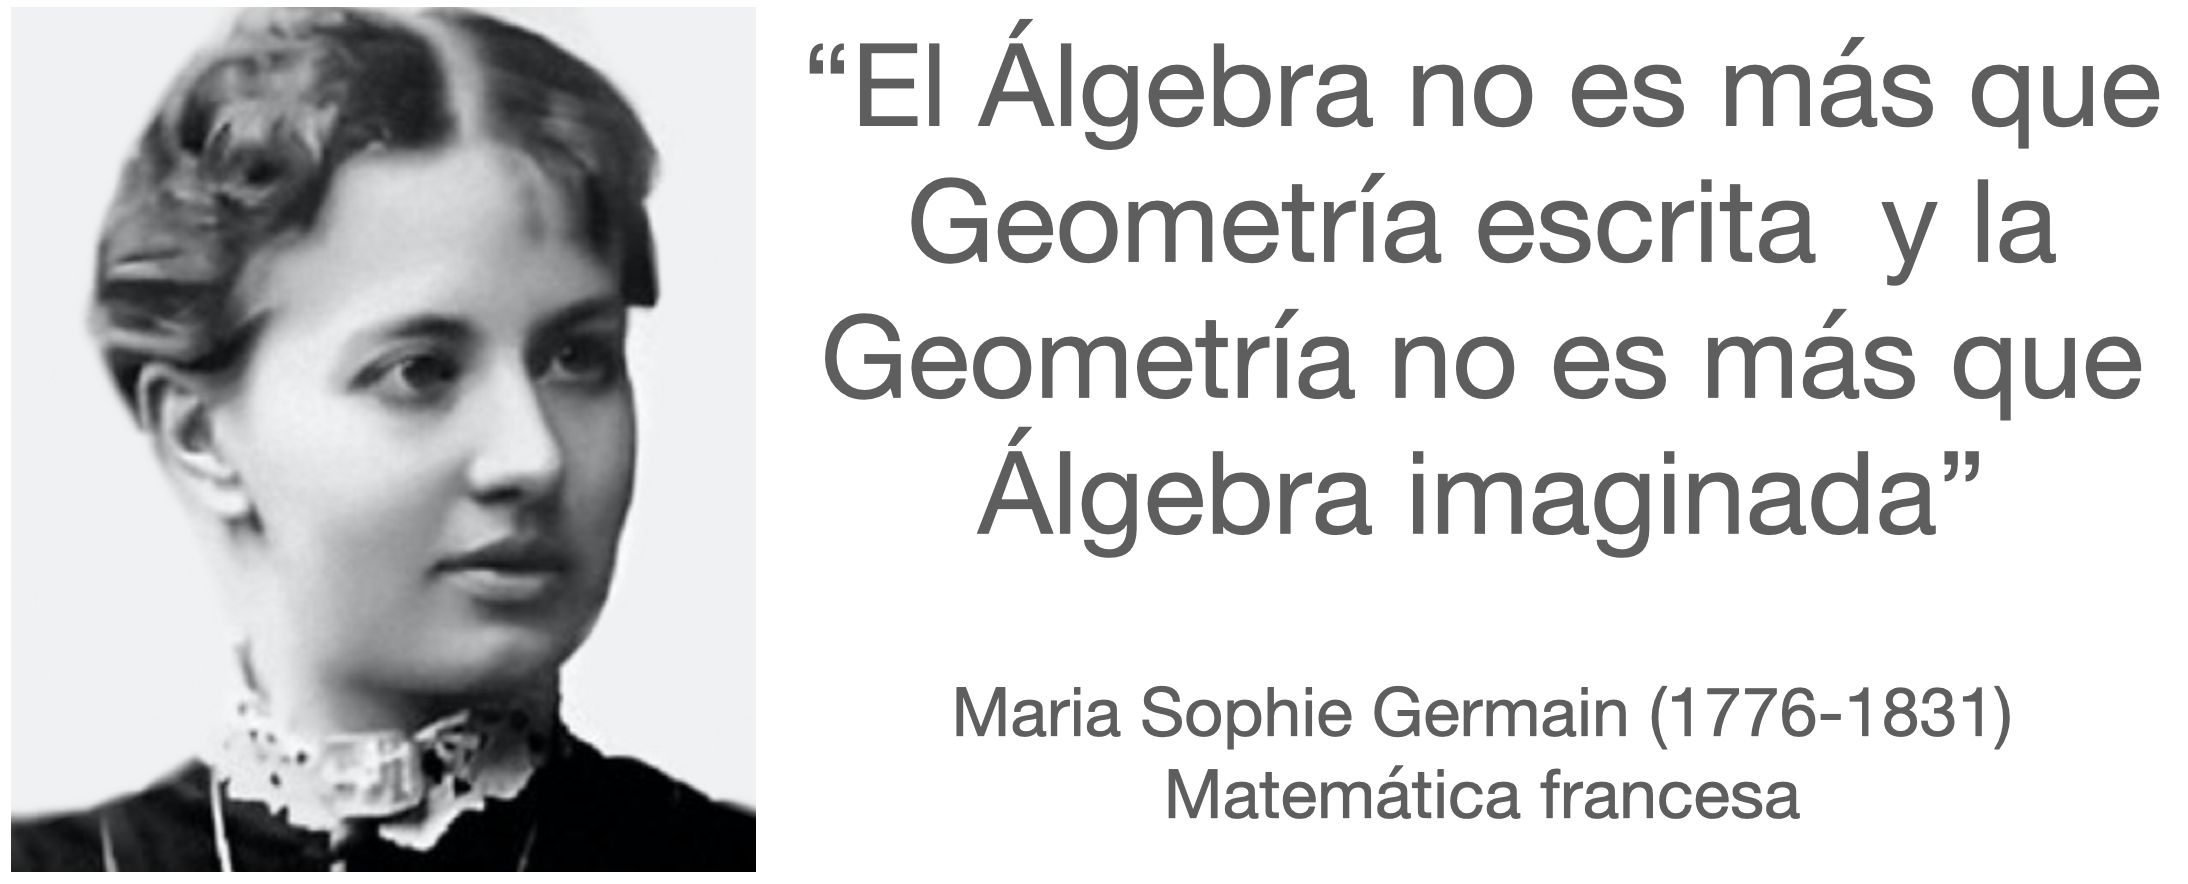
\includegraphics[width=.9\textwidth]{imagenes/imagenes09/Sophie-Germain.png}
	\end{figure}

\end{myblock}



\section[El espacio vectorial de los vectores libres del espacio]{El espacio vectorial de los vectores libres del espacio \sectionmark{E.V. de los Vectores libres}}

\sectionmark{E.V. de los Vectores libres}

$E_3=\{\text{conjunto puntos del espacio}\}=\{A, B, C, \cdots \}$

$V_3=\{\text{conjunto `vectores libres' del espacio}\}=\{\vec u, \vec v, \vec w, \cdots \}$

\normalsize{Las} definiciones que se dan a continuación se muestran en la figura siguiente.

\begin{defi}
Dados dos puntos fijos $A$ y $B$ del espacio de puntos $E_3$, se llama \textbf{`vector fijo'} $\overrightarrow {AB}$ al segmento orientado con origen en $A$ y extremo en $B$.	
\end{defi}

Dos puntos $A$ y $B$ determinan un solo segmento, $\overline{AB}=\overline{BA}$ y dos vectores fijos  $\overrightarrow {AB}$ y  $\overrightarrow {BA}$.

Un vector fijo se dice que es el vector nulo cuando su origen y extremo coinciden: $\boldsymbol{\vec 0}= \overrightarrow {AA} =\overrightarrow {BB} = \overrightarrow {CC}=\cdots$

\vspace{2mm} \begin{defi}{Características de un vector}

Además de extremo y origen, en un vector fijo podemos observar:

--- \textbf{Módulo} de un vector fijo $\overrightarrow {AB}$: es la longitud del segmento $\overrightarrow {AB}$ y se representa por  $|\overrightarrow {AB|}$


--- \textbf{Dirección} de un vector fijo $\overrightarrow {AB}$: es la determinada por la recta que pasa por los puntos $A$ y $B$ y todas las rectas paralelas a ella \textcolor{gris}{(todas las rectas paralelas tienen la misma dirección)}.

Dos vectores fijos  no nulos $\overrightarrow {AB}$ y  $\overrightarrow {CD}$ tienen la misma dirección si y solo si están situados sobre la misma recta o sobre rectas paralelas, se dice  que los vectores son paralelos: $\overrightarrow {AB}\; ||\; \overrightarrow {AB}$


--- \textbf{Sentido} de un vector fijo $\overrightarrow {AB}$: el que va desde el origen $A$ hasta el extremo $B$.

Toda dirección tiene dos sentidos. Em la figura, $\overrightarrow {AB}$ tiene el mismo sentido que $\overrightarrow {GH}$ pero sentido contrario a $\overrightarrow {CD}$: $\quad \overrightarrow {AB} \uparrow\uparrow \overrightarrow {GH}\; $; $\; \overrightarrow {AB} \uparrow \downarrow \overrightarrow {CD}$

\end{defi}

\begin{defi}{Vectores opuestos}

Dos puntos fijos del plano $A$ y $B$ determinan dos vectores $\overrightarrow {AB}$ y $\overrightarrow {BA}$ que se llaman \textbf{`opuestos'}.
	
\end{defi}

\begin{figure}[H]
	\centering
	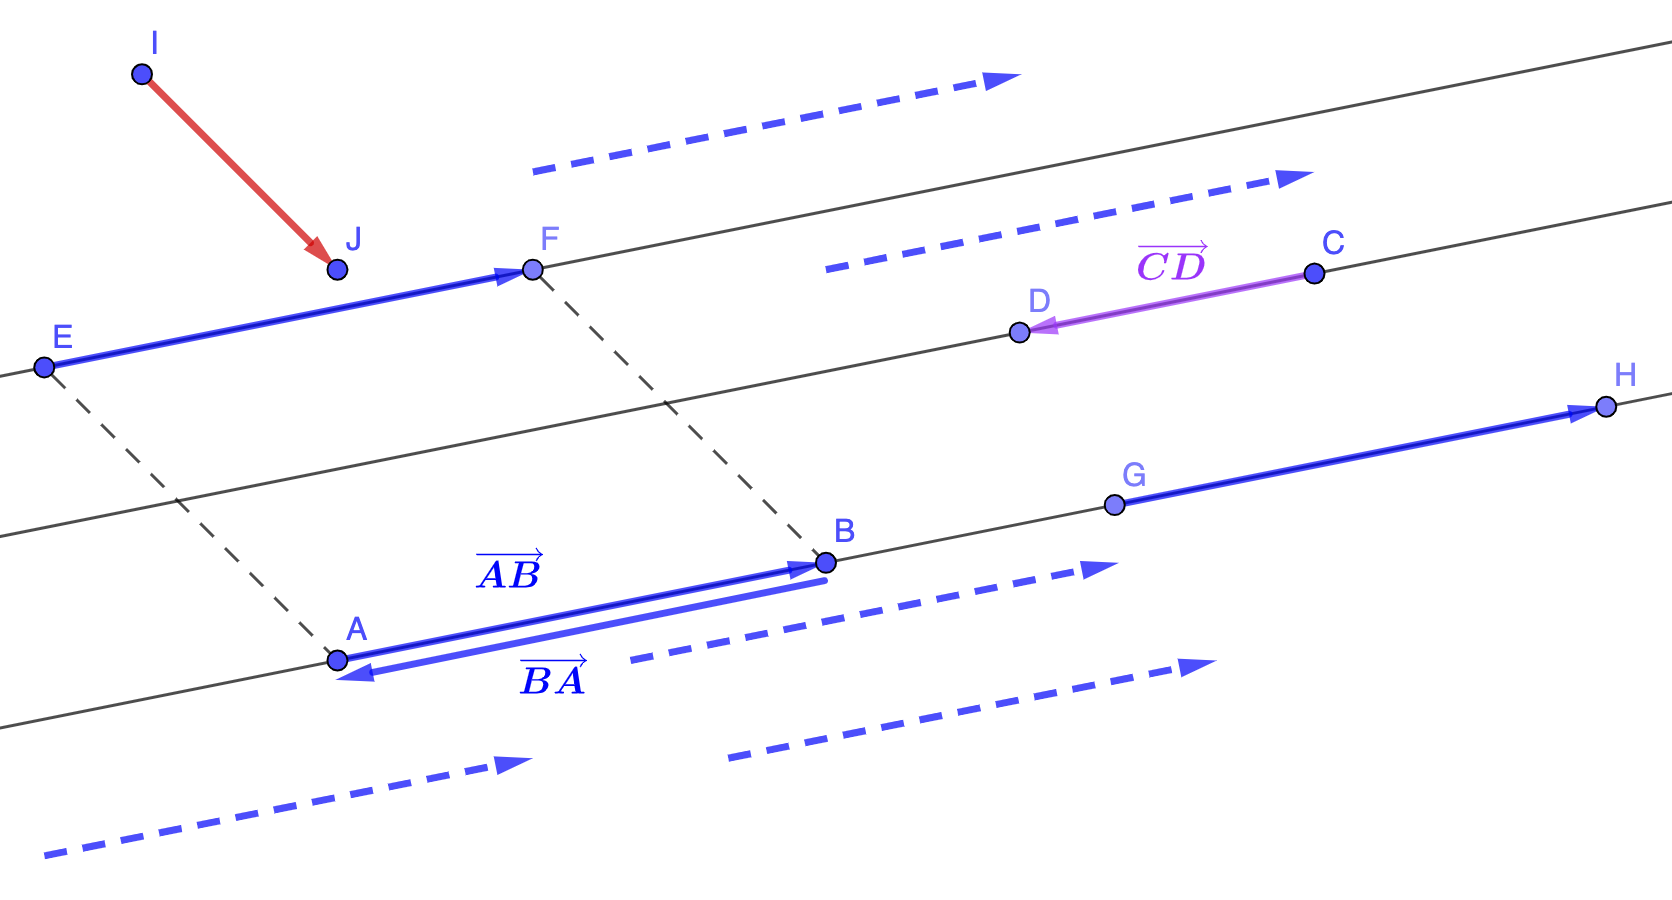
\includegraphics[width=.80\textwidth]{imagenes/imagenes09/T09IM01.png}
\end{figure}



Evidentemente, dos vectores fijos y opuestos tienen el mismo módulo, la misma dirección y sentidos contrarios:

$|\overrightarrow {AB}|=|\overrightarrow {BA}|; \quad \overrightarrow {AB}\; ||\; \overrightarrow {BA}; \quad \overrightarrow {AB} \uparrow\downarrow \overrightarrow {BA}$

\begin{defi}{Vectores equipolentes}

Dados dos vectores fijos $\overrightarrow {AB}$ y $\overrightarrow {GH}$ son `equipolentes' ($\overrightarrow {AB} \boldsymbol{\sim} \overrightarrow {GF}$) si tienen el mismo módulo, la misma dirección y el mismo sentido.
\end{defi}

En la figura anterior so observa que: 

$\overrightarrow {AB} \boldsymbol{\sim} \overrightarrow {GF} \;\; \longleftrightarrow \;\; 
|\overrightarrow {AB}|=|\overrightarrow {GH}| \;\; \wedge \;\; \overrightarrow {AB} \;||\; \overrightarrow {GH} \;\; \wedge \;\; \overrightarrow {AB} \uparrow\uparrow \overrightarrow {GH}$



\begin{prop}
	Si dos vectores fijos no nulos son equipolentes, entonces , o bien están en la misma recta ($\; \overrightarrow {AB} \text{ y } \overrightarrow {GH}\;$), es decir, $A,B,C,D$ están alineados, o bien el cuadrilátero $A,B,C,D$ obtenido al unir los orígenes y los extremos de los vectores se forma el `paralelogramo' $ABEF\; $ ($\; \overrightarrow {AB} \text{ y } \overrightarrow {EF}\;$). Ver figura anterior.
\end{prop}



\begin{defi}{\textbf{Vectores libres}}

Dado un vector fijo $\overrightarrow {AB}$, todos los vectores `equipolentes' a él definen el mismo \textbf{`vector libre'} $\boldsymbol{ \vec u }$ (dibujados en modo discontinuo en la figura anterior). $\vec u=\{\text{vector fijo } \overrightarrow {AB} \text{ y todos sus equipolentes} \}$

Al conjunto de todos los vectores libres del espacio $\mathbb R^3$ le llamamos $V_3$. 

`Módulo, dirección y sentido' de un vector libre es el módulo, dirección y sentido de uno cualquiera de sus vectores equipolentes.	
\end{defi}

Podemos considerar un `vector libre' como una \textit{flecha} que podemos dibujar con origen en cualquier punto con la única condición de no cambiar el tamaño (módulo), la dirección y el sentido.

Los vectores libres van a ser objetos matemáticos (de $V_3$) cuya función va a ser mover puntos (de $E_3$).

\subsection{Operaciones con vectores libres}

\subsubsection{--- Suma de vectores}

\begin{defi}
Dados $\vec u, \vec v \in V_3$, se define el vector suma, $\vec u + \vec v$	,  como aquel que se obtiene:

\begin{multicols}{2}
\begin{itemize}
\item `vectores concurrentes': dibujado el vector $\vec u$, con origen en su extremo dibujamos el vector $\vec v$. Entonces, el vector que va desde el origen de $\vec u$ hasta el extremo de $\vec v$ es el vector suma $\vec u + \vec v$.
\item `método del paralelogramos': dibujamos los vectores $\vec u$ y  $\vec v$  con el origen común (en el mismo punto de $E_3$) y construimos el paralelogramo formado por estos dos vectores (ver figura adjunta). Entonces, el vector suma, $\vec u + \vec v$, es el vector que sale del origen de ambos vectores y llega al extremo opuesto en la diagonal del paralelogramo.	
\end{itemize}

\begin{figure}[H]
	\centering
	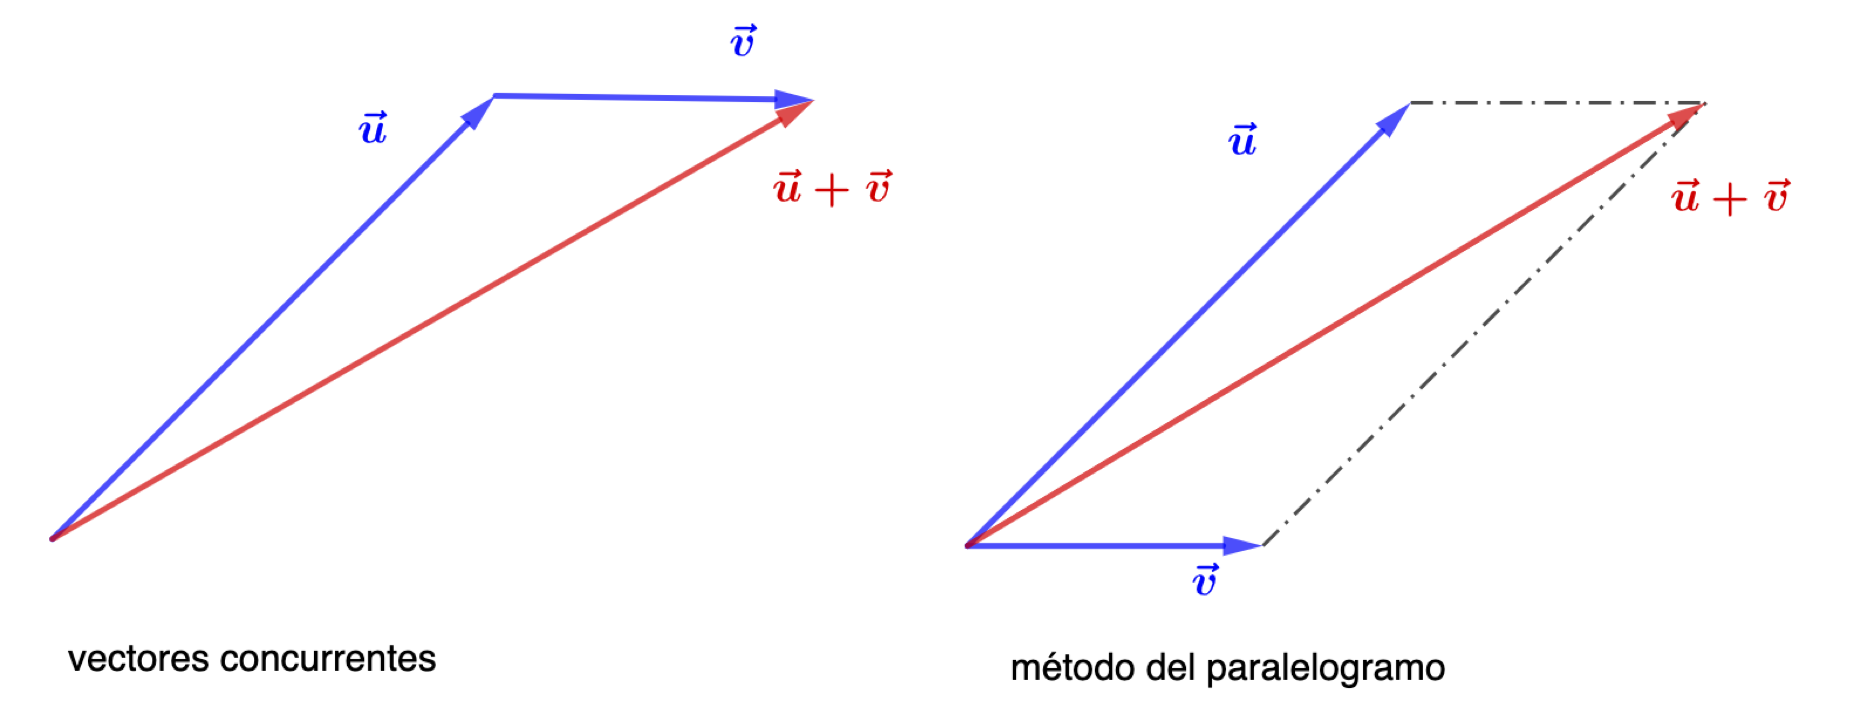
\includegraphics[width=.45\textwidth]{imagenes/imagenes09/T09IM02.png}
	\caption*{Suma de vectores libres}
\end{figure}

\end{multicols}
\end{defi}

\begin{prop}{Propiedades de la suma de vectores libres}

\begin{multicols}{2}
\begin{figure}[H]
	\centering
	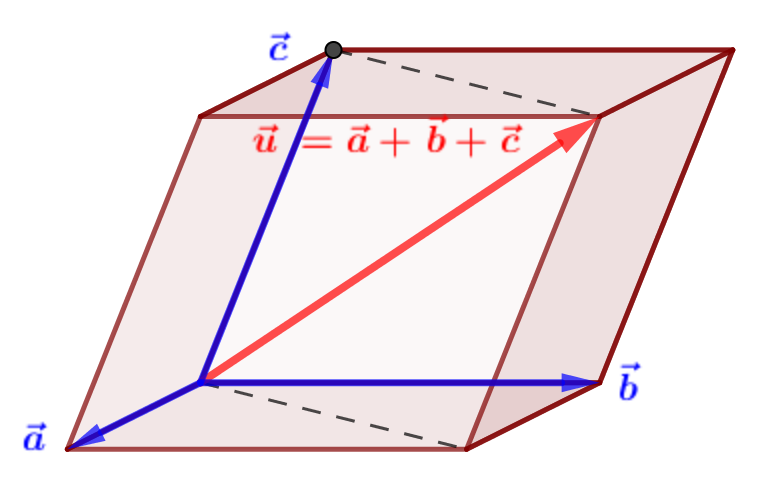
\includegraphics[width=.4\textwidth]{imagenes/imagenes09/T09IM02b.png}
\end{figure}
\begin{itemize}
\item \footnotesize{Conmutativa: $\vec u + \vec v=\vec v + \vec u$}
\item Asociativa: $\vec u + (\vec v+ \vec w)=(\vec u + \vec v)+\vec w$
\item Neutro: $\vec u + \vec 0=\vec 0+\vec u=\vec u$
\item Opuesto: $\vec u+ (\vec{-u})=(\vec{-u})+\vec u= \vec 0$
\end{itemize}
\end{multicols}
	\textcolor{gris}{\normalsize{Con} estas propiedades, $(V_3,+)$ tiene estructura algebraica de grupo abeliano (tema \ref{e_alg} de estructuras algebraicas).}
\end{prop}

\begin{defi}{Diferencia de vectores}
\begin{multicols}{2}
	Llamaremos diferencia (resta) de dos vectores a la suma del primero de ellos con el opuesto del segundo: 
	$\quad \vec u - \vec v = \vec u + (\vec {-v})$
	
\begin{figure}[H]
	\centering
	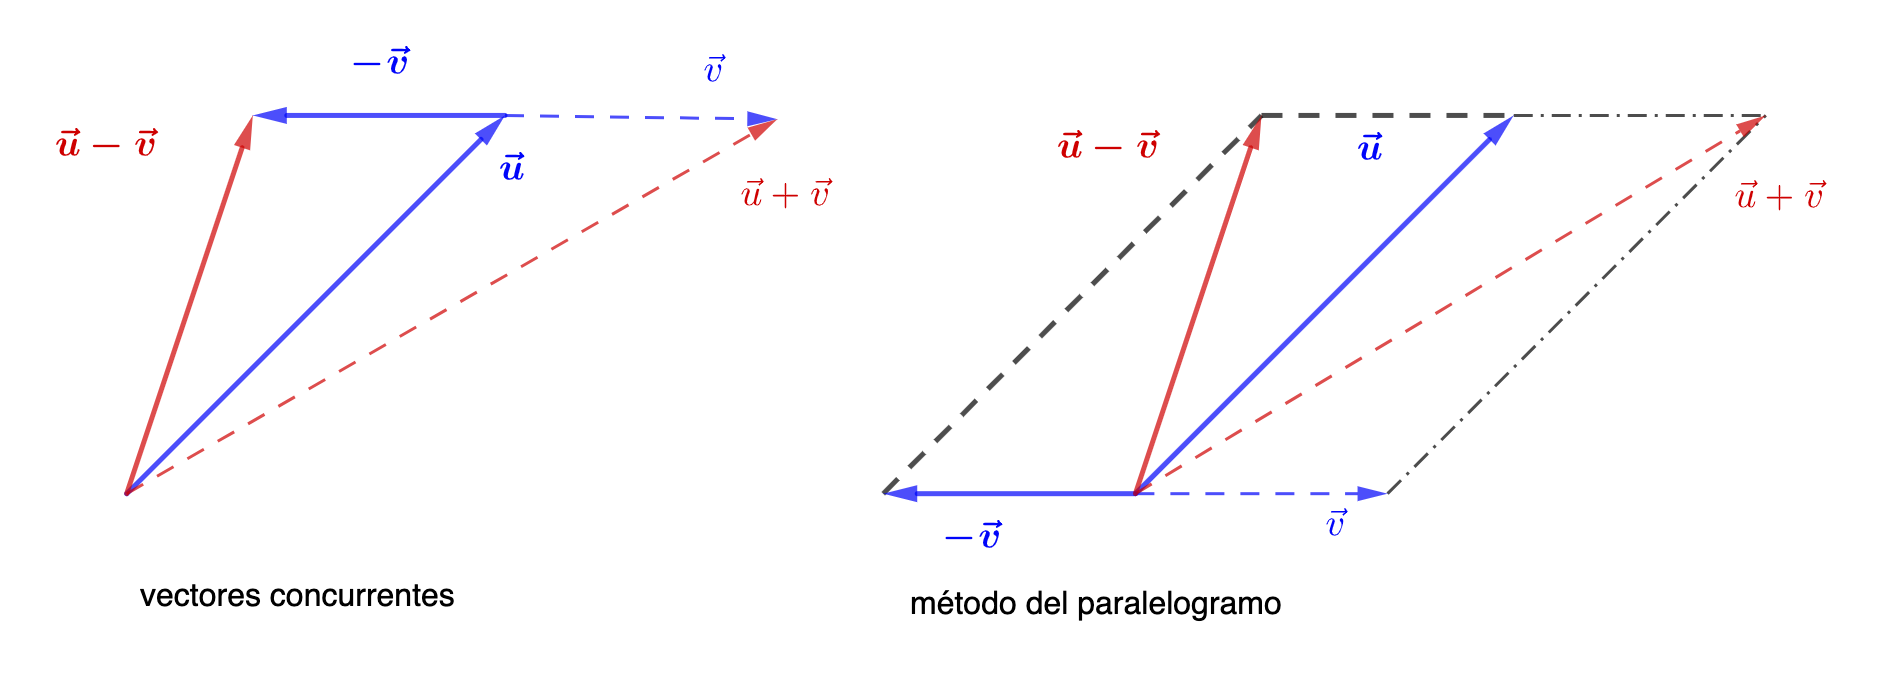
\includegraphics[width=.6\textwidth]{imagenes/imagenes09/T09IM03.png}
	\end{figure}
	
\end{multicols}
\end{defi}

\subsubsection{--- Producto de un vector libre por un escalar}

A los números reales, por contraposición a los vectores, se les llama `escalares'.

\begin{defi}

Sea $k\in \mathbb R; \; \vec u \in V_3$, se define el producto de $k$ por $\vec u$, como aquel vector $k \vec u$ que tiene por:

\tiny{$\blacksquare$} \normalsize{módulo}: $|k\vec u|= abs(k) \cdot mod(\vec u)=|k|\;|\vec u|$
\begin{multicols}{2}
\begin{itemize}
\item direción: la misma que $\vec u$
\item sentido: $\begin{cases} \text{ mismo que } \vec u \text{ si } k>0\\ \text{ contrario a } \vec u \text{ si } k<0	\end{cases} = \begin{cases} \; k\vec u \; \uparrow \uparrow \; \vec u \; \leftrightarrow \; k>0 \\ \; k\vec u \; \uparrow \downarrow \; \vec u \; \leftrightarrow \; k<0 \end{cases}$
\end{itemize}

\begin{figure}[H]
	\centering
	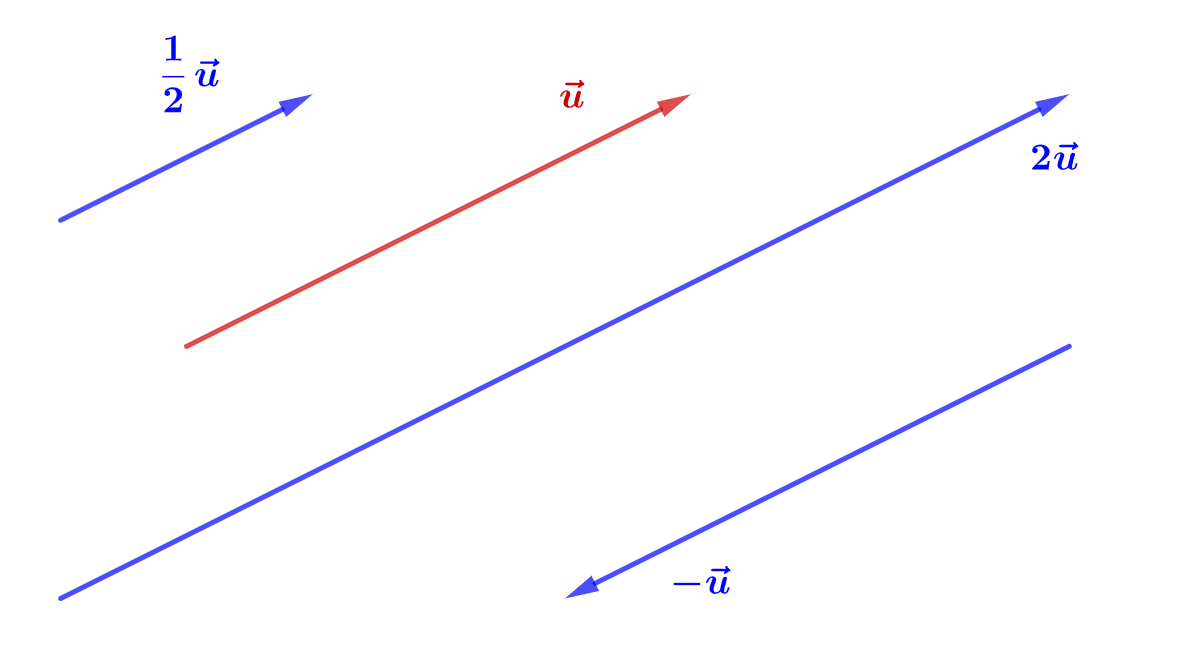
\includegraphics[width=.4\textwidth]{imagenes/imagenes09/T09IM04.png}
	\caption*{Producto por un escalar}
\end{figure}
\end{multicols}
	
\end{defi}

\begin{prop}{Propiedades del producto por un escalar}
\begin{multicols}{2}
\begin{itemize}
\item $k(\vec u + \vec v)=k \vec u + k \vec v$
\item $(k+h)\vec u=k\vec u + h\vec u$	
\item $(kh)\vec u=k(h\vec u)$
\item $1\vec u=\vec u$
\end{itemize}
\end{multicols}	
\textcolor{gris}{\normalsize{Con} estas propiedades, la terna $(V_3,+,\cdot)$ tiene estructura algebraica de espacio vectorial real (tema \ref{e_vec} de espacios vectoriales).}
\end{prop}

\subsection{Sistema de Referencia: coordenadas de un punto, componentes de un vector.}



$3$ vectores $\{ \; \vec u_1,\; \vec u_2, \; \vec u_3 \; \}$ de $V_3$ de distintas direcciones y no coplanarios son LI por lo que forman una \textbf{base} $B_{V_3}$: 

$\; \forall \vec u \in V_3\; \exists ! x \in \mathbb R, \; \exists ! y \in \mathbb R, \; \exists ! z \in \mathbb R\; \therefore \; \vec u=x\vec u_1+y \vec u_2+z \vec u_3$

\begin{defi}.

\begin{multicols}{2}
Llamaremos \textbf{Sistema de Referencia, $\boldsymbol{\mathcal R}$,} al concurso de un punto fijo del espacio de puntos, que llamaremos `origen', $\mathcal O \in E_3$ y una base del espacio vectorial $B=\{ \; \vec u_1,\; \vec u_2, \; \vec u_3 \; \}\subset V_3$, es decir: $\boldsymbol{\mathcal R = \{\; \mathcal O\; ; \;  \{ \; \vec u_1,\; \vec u_2, \; \vec u_3 \; \} \; \}}$

	\begin{figure}[H]
	\centering
	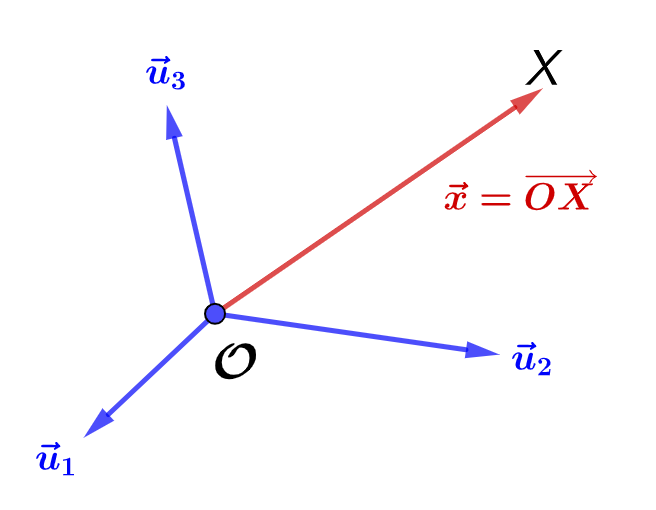
\includegraphics[width=.50\textwidth]{imagenes/imagenes09/T09IM05.png}
	\end{figure}
\end{multicols}

\begin{multicols}{2}
\begin{figure}[H]
	\centering
	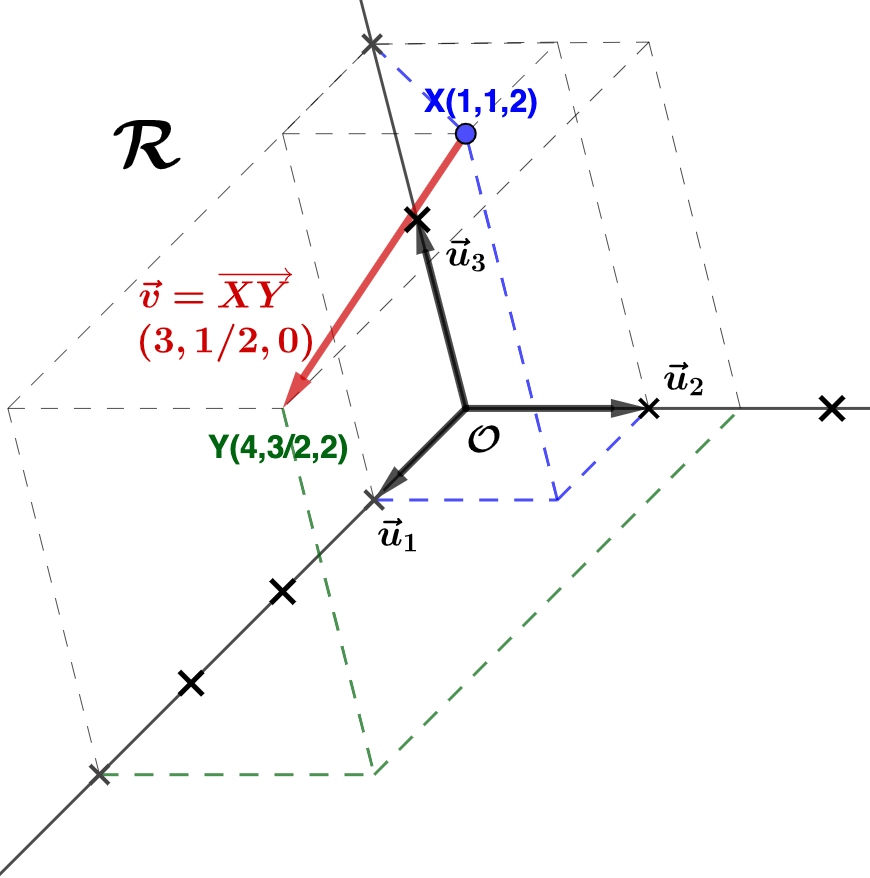
\includegraphics[width=.5\textwidth]{imagenes/imagenes09/T09IM06.png}
	\end{figure}

Para cualquier $X\in E_3$, hay un único vector que desde el origen $\mathcal O$ va hasta $X$, es el `vector de posición' del punto $X$, el vector $\vec x=\overrightarrow{OX}$.

$\vec x$, como vector que es, se escribe de forma única en la base $B$ de $\mathcal R$: $\; \vec x=\alpha \vec u_1 + \beta \vec u_2+ \gamma \vec u_3=(\alpha, \beta, \gamma)$ son las \textbf{componentes} del vector $\vec x$ en $\mathcal R$.
\end{multicols} 

$X$, como punto se puede escribir a través de su vector de posición como $X=(\alpha, \beta, \gamma)$ y ahora hablamos de las \textbf{coordenadas} de $X$ en $\mathcal R$.

\end{defi}


Si dibujamos $\vec v=(v_1,v_2,v_3)$ con origen en $X(x_1,x_2,x_3)$, su extremo será el punto $Y(y_1,y_2,y_3)$ cuyas componentes son $Y(x_1+v_1,x_2+v_2,x_3+v_3)$. De otro modo, llamando $\vec v=\overrightarrow{XY}$ :

$Coord\; Y= Coord\; X + Componentes \; \overrightarrow{XY} \quad $
\colorbox{LightYellow}{$\;\boxed{ \;\boldsymbol{\;Y=X+\overrightarrow{XY}\;\; }} $}

El vector $\vec v=\overrightarrow{XY}$ se desplaza $+3$ veces según el vector $\vec i$ (hacia delante del observador/a), $+1/2$  veces según el vector $\vec j$ (hacia la derecha) y $0$ veces según el vector $\vec k$ (hacia arriba). 

El trabajo de los vectores va a ser desplazar puntos. Al punto $X$ le aplicamos el vector $\vec v=\overrightarrow{XY}$ y lo desplazamos hasta la posición $Y$.



\begin{multicols}{2}
\noindent \textbf{NOTA}: Mientras no se diga lo contrario, las coordenadas del origen será $\mathcal O=(0,0,0)$ y la base que usaremos será la base canónica de $V_3$, formada por los vectores $C_{V_3}=\{\boldsymbol{\vec i}=(1,0,0);\;\boldsymbol{\vec j}=(0,1,0);\;\boldsymbol{\vec k}=(0,0,1)\}$, que forman una base llamada \textbf{`ortonormal'}, sus módulos valen $1$ (`normal'-izado) y son mutuamente perpendiculares (`ortogonales): $\vec i \bot \vec j; \; \vec j \bot \vec k; \; \vec k \bot \vec i$

	\begin{figure}[H]
	\centering
	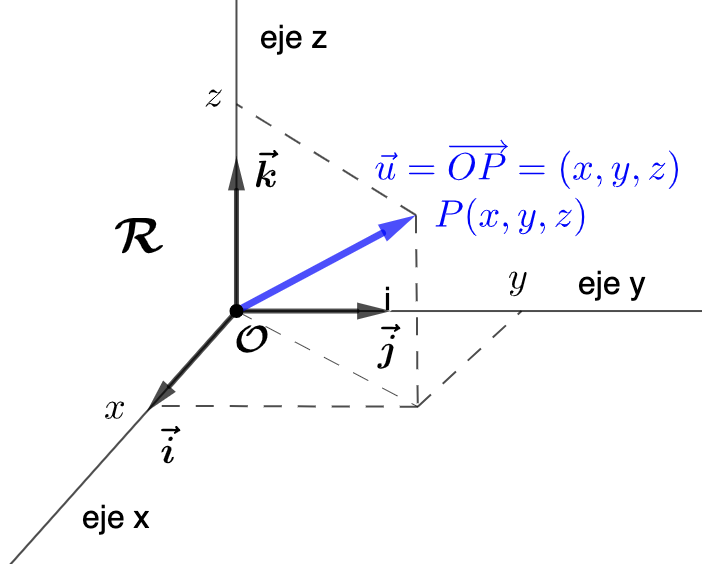
\includegraphics[width=.5\textwidth]{imagenes/imagenes09/T09IM07.png}
	\end{figure}
\end{multicols}

\begin{ejem}

En la siguiente figura, encuentra las coordenadas de los puntos $A,B,C,D,E,F,P$ y del vector $\vec u=\overrightarrow{OP}$	
\end{ejem}

%\clearpage

\begin{multicols}{2}

	\begin{figure}[H]
	\centering
	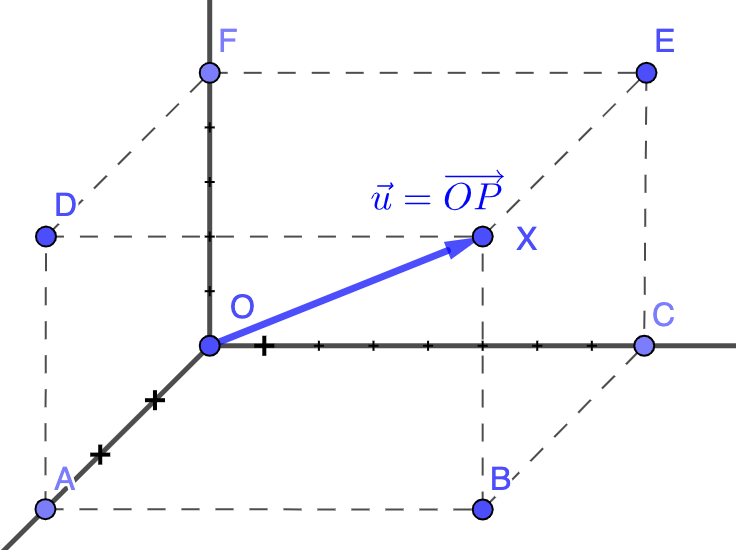
\includegraphics[width=.50\textwidth]{imagenes/imagenes09/T09IM08.png}
	\end{figure}
	
	\textcolor{gris}{$A(3,0,0)\; B(3,8,0); \; C(0,8,0)$}
	
	\textcolor{gris}{$D(3,0,5);\; E(0,8,5); \; F(0,0,5)$}
	
	$\quad$
	
	\textcolor{gris}{$X(3,8,5)$}
	
	\textcolor{gris}{$\vec u=\overrightarrow{OX}=(3,8,5)=3\vec i+8\vec j+5 \vec k$}

\end{multicols}

\subsection{Aplicaciones de los vectores}

\textbf{Componentes del vector que une dos puntos}

\begin{multicols}{2}

	\begin{figure}[H]
	\centering
	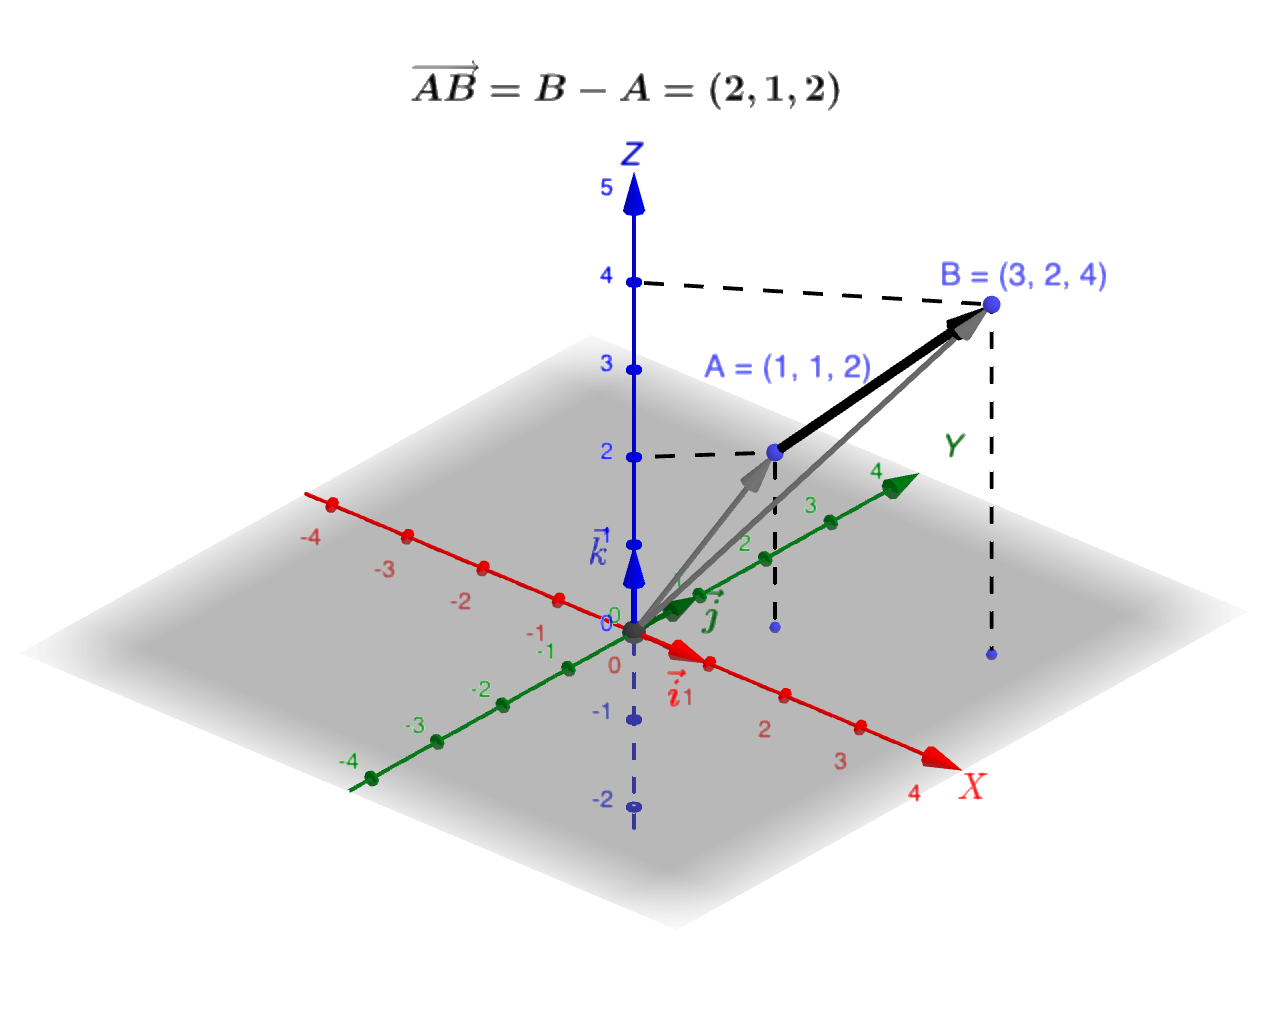
\includegraphics[width=.55\textwidth]{imagenes/imagenes09/T09IM09.png}
	\end{figure}
	
	$\mathcal R\{\mathcal O; \vec i, \vec j, \vec k\}$ sistema de referencia ortonormal, en que $A(a_x,a_y,a_z)$ y $B(b_x,b_y,b_z)$
son las coordenadas de dos puntos. De la figura se observa que:

\noindent $\overrightarrow{OA}+\overrightarrow{AB}=\overrightarrow{OB} \to \overrightarrow{AB}=\overrightarrow{OB}-\overrightarrow{OA}$

\noindent \footnotesize{$A\to \overrightarrow{OA}=(1,1,2); \; B\to \overrightarrow{OA}=(3,2,4)$}

\noindent \normalsize{$\overrightarrow{BA}=B-A=(2,1,2)$}

\end{multicols}



\noindent \small{$\overrightarrow{AB}=\overrightarrow{OB}-\overrightarrow{OA}$}\normalsize{,} abusando del lenguaje podemos decir que: \colorbox{LightYellow}{$\boxed{\; \overrightarrow{AB}=B-A\;}$}, para calcular las componentes, en un sistema de referencia dado, del  vector que representa (une) dos puntos bastará con restar a las coordenadas del punto extremo, las coordenadas del punto origen: \textit{`componentes del vector que une dos puntos = coordenadas del extremo menos coordenadas del origen'.}

Repitiendo lo dicho más arriba, si $\overrightarrow{AB}=B-A$, `despejando' $B=A+\overrightarrow{AB}$  y tenemos, como se ha mencionado anteriormente, que el trabajo de los vectores va a ser desplazar puntos. Al punto $A$ le aplicamos el vector $\overrightarrow{AB}$ y lo desplazamos hasta la posición $B$.

$\mathcal R\{\mathcal O; \vec i, \vec j, \vec k\}$ sistema de referencia ortonormal, las coordenadas del punto $A(a_x,a_y,a_z)$ coinciden con las componentes del vector de posición $\overrightarrow{OA}=a_x\vec i+a_y \vec j+ a_z\vec k=(a_x,a_y,a_z)$, análogamente $B(b_x,b_y,b_z)$ por ser $\overrightarrow{OB}=b_x\vec i + b_y\vec j+b_z\vec k=(b_x,b_y,b_z)$. Las componentes del vector que une los dos puntos, desde $A$ hasta $B$ las obtendremos, abusando del lenguaje, al restar de las coordenadas del extremo $B$ las coordenadas del origen $A$. Decimos abusando del lenguaje porque, evidentemente dos puntos no se pueden restar, lo que hacemos en realidad es definir $\overrightarrow{AB}=\overrightarrow{OB}-\overrightarrow{OB} $ aunque en la  práctica haremos: $\boldsymbol{\overrightarrow{AB}=B-A}$

\vspace{5mm} \textbf{Condición de paralelismo de dos vectores}

De la definición de producto de un vector por un escalar sabemos que el resultado son vectores paralelos, es decir: $\vec u \; || \; \vec v \; \leftrightarrow \; \exists k \in \mathbb R\; / \; \vec u = k\cdot \vec v$

Si $\vec v=(v_x,v_y,v_z) \quad \to \quad k\cdot u=(kv_z,k_vy,kv_z)=(u_x,u_y,u_z) \quad \longrightarrow \quad u_x=kv_x; \;u_y=kv_y; \;u_z=kv_z$, es decir, \textit{\colorbox{LightYellow}{dos vectores son paralelos si sus} \colorbox{LightYellow}{componentes son proporcionales.}} $\quad \dfrac {\vec u_x}{\vec v_x}=\dfrac {\vec u_y}{\vec v_y}=\dfrac {\vec u_z}{\vec v_z}=k$
	
\vspace{3mm} \textbf{Condición de puntos alineados}

\begin{multicols}{2}
Tres puntos $A,\;B$ y $C$ están alineados si, formados dos vectores cualesquiera con ellos tres, éstos resultan paralelos: $\overrightarrow{AB}\;||\;\overrightarrow{AC}$

\begin{figure}[H]
	\centering
	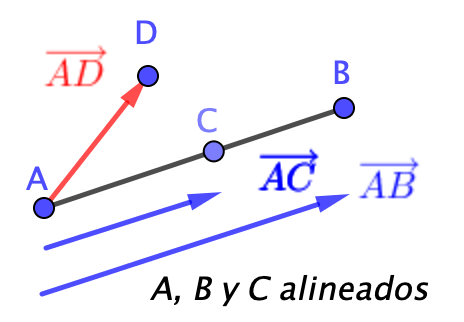
\includegraphics[width=.35\textwidth]{imagenes/imagenes09/T09IM14.png}
\end{figure}
\end{multicols}

\vspace{-5mm} \textbf{Punto medio de un segmento}

\begin{multicols}{2}
Dado el segmento $\overline{AB}$, llamamos ' punto medio' del segmento al punto  $M$ que verifica la ecuación: $\; \overrightarrow{AM}=\frac 1 2 \overrightarrow{AB}\; $

Sean $A(a_x,a_y,a_z); \; B(b_x,b_y,b_z)$ las coordenadas de $A$ y $B$ extremos del segmento, entonces, las coordenadas de $M(m_x,m_y,m_z)$ se pueden escribir como: $m_i=\frac {a_i+b_i}{2},\; \text{ con } i=\{x,y,z\}$

\begin{figure}[H]
	\centering
	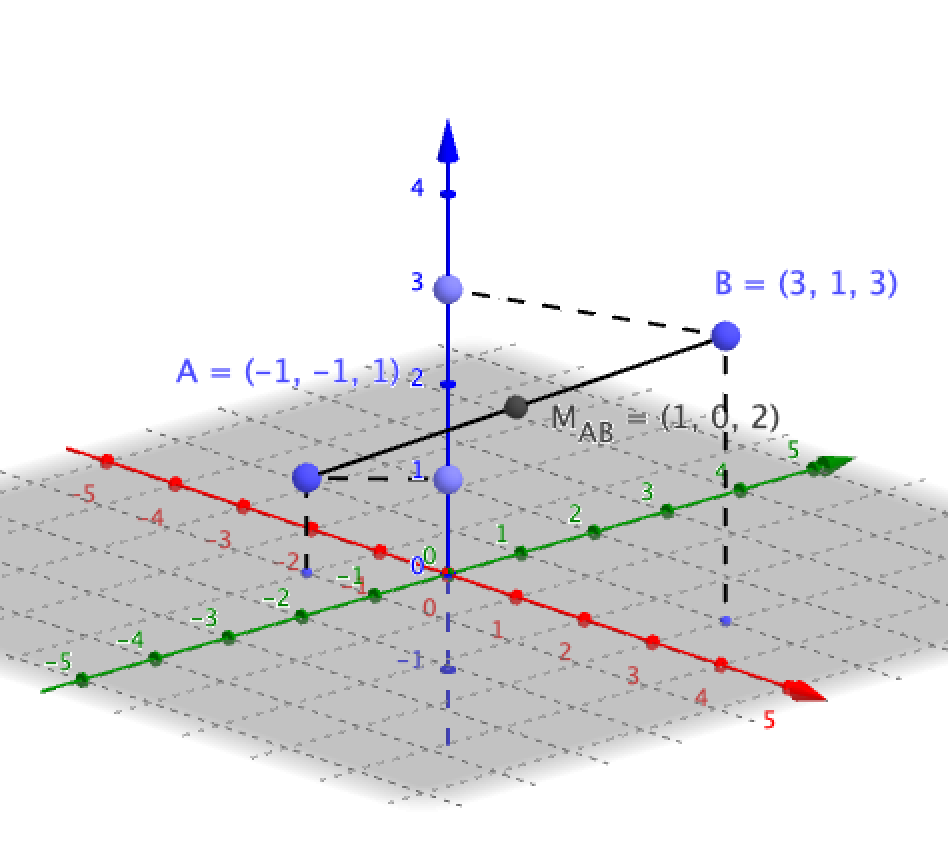
\includegraphics[width=.55\textwidth]{imagenes/imagenes09/T09IM10.png}
\end{figure}
\end{multicols}

\noindent \footnotesize{\textcolor{gris}{$\overrightarrow{AM}=\frac 1 2 \overrightarrow{AB} \to (m_x,m_y,m_z)-(a_x,a_y,a_z)=\frac 1 2 [\;(b_x,b_y,b_z)-(a_x,a_y,a_z)\;]$, despejando, $m_i=\frac {a_i+b_i}{2},\; \text{ con } i=\{x,y,z\}$}}\normalsize{.}

\textit{Las `coordenadas del punto medio' de un segmento las obtendremos como `semisuma de las coordenadas de los extremos'}: \colorbox{LightYellow}{$\; \boxed{\; M_{AB}=\dfrac {A+B}{2}\; }\; $}

\vspace{5mm}\textbf{Simétrico de un punto $\boldsymbol{P}$ respecto de otro  $\boldsymbol{Q}$}
\begin{multicols}{2}
\begin{figure}[H]
	\centering
	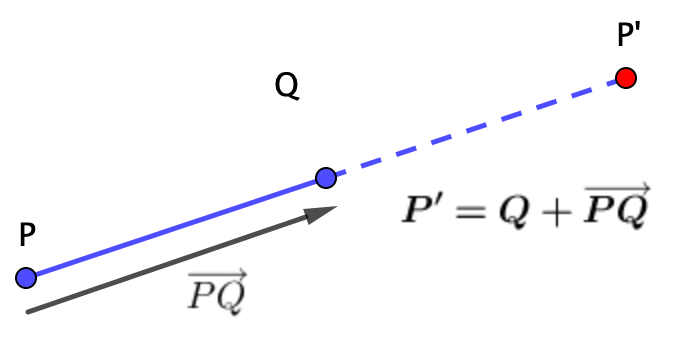
\includegraphics[width=.45\textwidth]{imagenes/imagenes09/T09IM12.png}
\end{figure}
Dados $P$ y $Q$, el simétrico de $P$ respecto de $Q$ ha de ser un punto $P'$ tal que $Q$ sea el punto medio del segmento $\overline{PP'}$.


\end{multicols}
Es decir, $P'=Q+\overrightarrow{PQ}$, en coordenadas: \colorbox{LightYellow}{$\boxed{\;\dfrac {P+P'}{2}=Q \to P'=2Q-P\;}$} \textcolor{gris}{(abusando del lenguaje)}

\vspace{5mm} \textbf{División de un segmento en $\boldsymbol{ n }$ partes.}

\begin{multicols}{2}

Dados los puntos $A$ y $B$, formamos el vector $\overrightarrow{AB}$ y, a partir de él, $\frac 1 n \overrightarrow{AB}$. Si a $A$ le sumamos este último vector llegamos al punto $A_1=A+\frac 1 n \overrightarrow{AB}$; análogamente, $A_2=A+\frac 2 n \overrightarrow{AB}$ y, en general, 
\begin{figure}[H]
	\centering
	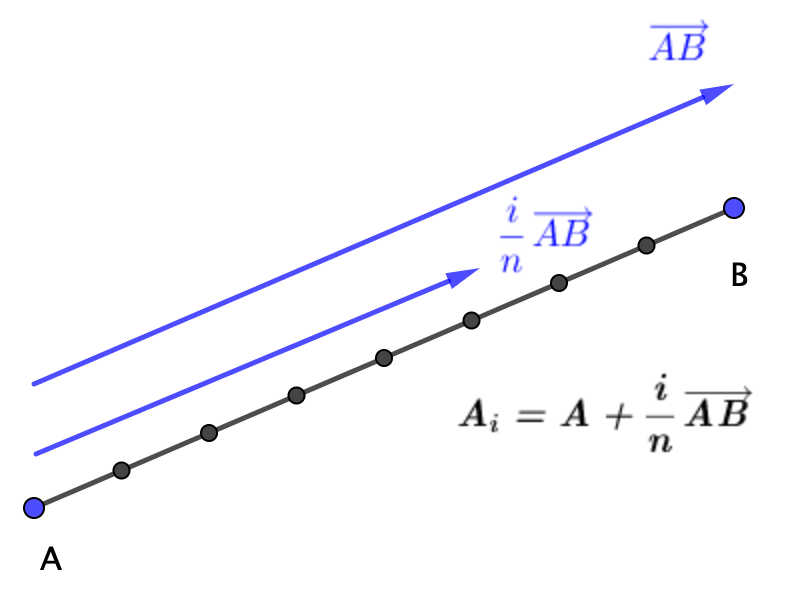
\includegraphics[width=.45\textwidth]{imagenes/imagenes09/T09IM11.png}
\end{figure}

\end{multicols}
\colorbox{LightYellow}{$\boxed{\;A_i=A+\frac i n\;  \overrightarrow{AB}\;}$}. $\quad$ Evidentemente, $A_0=A; \; A_n=B$

\newpage %*****************************************************
\textbf{Baricentro de un triángulo}

\begin{multicols}{2}
\begin{figure}[H]
	\centering
	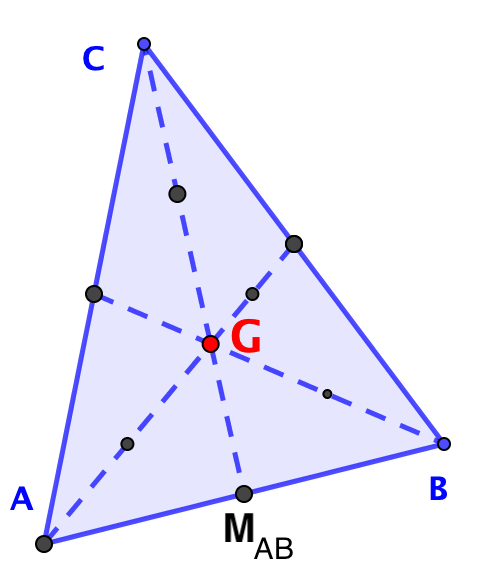
\includegraphics[width=.35\textwidth]{imagenes/imagenes09/T09IM13.png}
\end{figure}

$3$ puntos no alineados $A,B, C$ definen un triángulo. Se llama `baricentro' o `centro de gravedad' de un triángulo, $G$,  al corte de sus medianas \textcolor{gris}{(mediana: recta que va de un vértice de un triángulo al punto medio del lado opuesto; el baricentro dista del vértice el doble que del punto medio)} 

\end{multicols}

De nuevo abusando del lenguaje, se tiene que: \colorbox{LightYellow}{$\boxed{\;G=\frac{A+B+C}{3}\;}\; .$\; }
El baricentro, $G$,  de un triángulo está en la `tercisuma' de sus vértices:



\vspace{3mm}En lo sucesivo usaremos la siguiente \underline{notación}: $\boldsymbol{ P(x,y,z)}$, para los \textbf{puntos} usaremos letras mayúsculas y escribiremos sus componentes sin el símbolo igual, $\boldsymbol{\vec u=(u_x,u_y,u_z)}$, para los  \textbf{vectores} usaremos letras minúsculas, con flechita arriba, y sus componentes las escribiremos después del signo igual.

\begin{ejem}
\small{Considera} los puntos $A(1,2,-3),$ $\; B(4,5,0),$ $\; C(-2,5,3)$ y $D(3,x,-1)$. Se pide:
\begin{enumerate}[a) ]	
\item $\overrightarrow {AB}$ y  $\overrightarrow {BA}$
\item Comprueba que $\overrightarrow {AB}+\overrightarrow {BC}=\overrightarrow{AC}$ 
\textcolor{gris}{(Ley de Chasles)} y que 
$\overrightarrow {AB}+\overrightarrow {BC}+\overrightarrow {CA}=\overrightarrow {0}$
\item Determina el valor de $x$ en $D$ para que $A,B$ y $D$ estén alineados.
\item Idem para  $\overrightarrow {AB}\;||\;\overrightarrow {CD}$	
\item Encuentra el punto medio del segmento  $\overline {AB}$
\item Encuentra las coordenadas de un punto $P$ del segmento  $\overline {AB}$ tal que la distancia a $B$ sea doble que la distancia a $A$
\item Encuentra el baricentro del triángulo de vértices $A,B,C$
\item Comprueba que la distancia del baricentro a un vértice del triángulo es doble que la de éste al punto medio del lado opuesto al vértice.
\end{enumerate}
%\normalsize{---------------------------}

\small{\noindent --- a) $\overrightarrow {AB}=B-A=(3,3,3);\quad \overrightarrow {BA}=A-B=(-3,-3,-3)$, evidentemente, $\overrightarrow {BA}=-\overrightarrow {AB}$}

\noindent --- b) $\overrightarrow {AB}=(3,3,3); \; \overrightarrow {BC}=C-B=(-6,0,3); \; \overrightarrow {AB}+\overrightarrow {BC}=(3,3,3)+(-6,0,3)=(-3,3,6)$

\noindent Por otro lado: $\overrightarrow {AC}=C-A=(-3, 3, 6)$. 

\noindent Luego sí se cumple que $\overrightarrow {AB}+\overrightarrow {BC}=\overrightarrow{AC}$

\noindent --- c) $A,B$ y $D$ están alineados si $\overrightarrow {AB}\;||\;\overrightarrow {AD}$:

\noindent $\overrightarrow {AB}=(3,3,3); \; \overrightarrow {AD}=D-A=(2,x-2,2) \to \frac 2 3 = \frac {x-2} 3 = \frac 2 3 \to x=4$

\noindent --- d) $\overrightarrow {AB}\; ||\; \overrightarrow {CD}$ si sus componentes son proporcionales:

\noindent $\overrightarrow {AB}=(3,3,3); \; \overrightarrow {CD}=D-C=(5, x-5, -4) \to \frac 5 3 = \frac {x-5} 3 =\frac {-4} 3$, evidentemente, $\frac 5 3 \neq \frac {-4} 3 \Rightarrow \nexists \; x\; / \; \overrightarrow {AB}\;|| \; \overrightarrow {CD}$ 

\noindent --- e) $M_{AB}=\dfrac {A+B} 2 = \dfrac {(5,7,-3)}2=(5/2, 7/2, -3/2)$

\noindent --- f) De la figura: 
\begin{multicols}{2}
\noindent$P=A+\frac 2 3 \overrightarrow {AB}$

\noindent$P=(1,2,-3)+\frac 2 3 (3,3,3)$

\noindent$P=(1,2,-3)+(1,1,1)=(2,3,2)$
\begin{figure}[H]
	\centering
	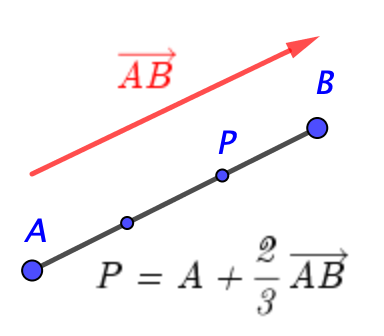
\includegraphics[width=.3\textwidth]{imagenes/imagenes09/T09IM15.png}
\end{figure}
\end{multicols}

\vspace{-8mm}
\noindent --- g) $G=\dfrac {A+B+C} 3 =\dfrac {(3,14,0)} 3 = (1,4,0)$

\noindent --- h) Fijándonos en la figura del apartado `baricentro', se observa que: $G=M_{AB}+\frac 1 3 \overrightarrow{M_{AB}C} \; (*)$

\noindent $M_{AB}=(5/2,7/2,-3/2); \; \overrightarrow{M_{AB}C}=C-M_{AB}=(-2,5,3)-(5/2,7/2,-3/2)=(-9/2,3/2,9/2)$

\noindent $(*)\to G=(5/2,7/2,-3/2)+\frac 1 3 (-9/2,3/2,9/2)=(5/2,7/2,-3/2)+(-3/2,1/2,3/2)=(1,4,0)$, obviamente, el mismo resultado anterior $\qquad \qquad \qquad \qquad \Box\qquad $ \normalsize{.}

\end{ejem}

Vamos ahora a estudiar tres diferentes productos con vectores, el producto escalar, el producto vectorial y el producto mixto, todos ellos con importantes aplicaciones geométricas.
\section{Producto escalar}\label{prodesc}

\begin{defi}
Dados $\vec u, \vec v \in V_3$, se define el producto escalar de dos vectores como el número real (escalar): \colorbox{LightYellow}{$\boxed{\; \vec u \cdot \vec v=|\vec u|\;|\vec v|\; \cos \theta\; }$}$\; \in \mathbb R$, siendo $\theta$ el ángulo que forman $\vec u \text{ y } \vec v$	
\end{defi}

\begin{multicols}{2}
\noindent Interpretación geométrica del producto escalar:

\noindent $\vec u \cdot \vec v=|\vec u|\;|\vec v|\; \cos \theta=|\vec u|\; Proy_{\;\vec u}\;(\vec v)$; 

\noindent siendo $Proy_{\; \vec u}\;(\vec v)=|\vec v|\; \cos \theta$

\begin{figure}[H]
	\centering
	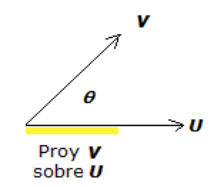
\includegraphics[width=.3\textwidth]{imagenes/imagenes09/T09IM16.png}
\end{figure}
\end{multicols}

\vspace{-5mm} El producto escalar de dos vectores es el módulo de uno de ellos por la proyección del otro sobre él.

\begin{prop}{Propiedad fundamental del producto escalar}

\vspace{3mm} \centerline{\colorbox{LightYellow}{$\; \vec u \; \bot \; \vec v \;  \longleftrightarrow \; \vec u \cdot \vec v = 0\; $}}	
\end{prop}
\justify
\vspace{-3mm} \begin{proofw}
$\boxed{\rightarrow} \quad$	Si $\vec u \; \bot \; \vec v  \longrightarrow \theta=90^o \longrightarrow \vec u \cdot \vec v=|\vec u|\;|\vec v|\; \cancelto{0}{cos (90^o)}=0$

\noindent $\boxed{\leftarrow} \quad$	 Si $\vec u \cdot \vec v = 0$  \scriptsize{y $\vec u\neq \vec 0\; \wedge \; \vec v \neq 0$}  \normalsize{$\to$}  $|\vec u|\;|\vec v|\; \cos \theta=0 \to \cos \theta=0 \longrightarrow $

\noindent $\theta =90^o:\; \vec u \; \bot \; \vec v$
\end{proofw}

\noindent \textbf{Propiedades del producto escalar:}

\noindent $\vec u \cdot \vec v=\vec v \cdot \vec u; \quad \alpha (\vec u \cdot \vec v)=(\alpha \vec u) \cdot \vec v= \vec u \cdot (\alpha \vec v); \quad  \vec u \cdot (\vec v\ + \vec w)= \vec u \cdot \vec v+ \vec u \cdot \vec w$


\noindent \textbf{Aplicaciones del producto escalar:}

\textbf{Módulo de un vector:}

$\vec u \cdot \vec u=|\vec u|\; |\vec u|\; \cancelto{1}{\cos\; 90^o}=|\vec u|^2 \quad \longrightarrow \qquad  \boldsymbol{ |\vec u|=+\sqrt{\vec u \cdot \vec u} }$

\textbf{Ángulo de dos vectores}

$\vec u \cdot \vec v=|\vec u|\;|\vec v|\; \cos \theta \quad \longrightarrow \qquad \boldsymbol{ \cos \theta = \dfrac {\vec u \cdot \vec v}{|\vec u|\; |\vec v|} }$

\textit{Es por esto por lo que muchos autores hablan del producto escalar como la `métrica' del espacio, pues nos permite medir distancias (módulos) y ángulos. Podríamos decir que el producto escalar es la cinta métrica y el goniómetro (transportador) del matemático.}

\begin{multicols}{2}
Aunque parezca existir una cierta ambigüedad a la hora de definir el ángulo que forman dos vectores, pues dado $\cos \theta$ igual a un determinado valor existen dos ángulos posibles $\theta$ y $360^o-\theta$ que lo verifican, la ambigüedad desaparece al definir el ángulo entre dos vectores como el menor de los dos posibles (menor de $180^o$).
\begin{figure}[H]
	\centering
	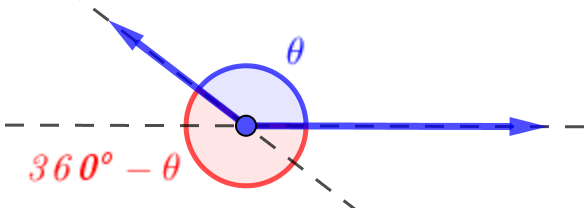
\includegraphics[width=.45\textwidth]{imagenes/imagenes09/T09IM17.png}
\end{figure}
\end{multicols}

\subsection{Expresión del producto escalar en una BON (base ortonormal)}

\begin{prop}
Sea $B=\{ \;  \vec i;\; \vec j;\; \vec k\; \; \therefore \;  \; |\vec i|=|\vec j|=|\vec k|=1 \; \text {  y  } \; \vec i \bot \vec j; \; \vec j \bot \vec k; \; \vec k \bot \vec i \; \}$, una BON y $\vec u,\; \vec v$ dos vectores de $V_3$ cuyas componentes en la BON son:  $\vec u=u_x\vec i+u_y\vec j+u_z\vec k=(u_x,u_y,u_z);\; \; \vec v=v_x\vec i+v_y\vec j+v_z\vec k=(v_x,v_y,v_z)$, se demuestra que:

$\boldsymbol{\vec u \cdot \vec v = u_xv_x+u_yv_y+u_zv_z} \quad \in \mathbb R$

$\boldsymbol{|\vec u|}= + \sqrt{\vec u \cdot \vec u}=\boldsymbol{+\sqrt{u_x^2+u_y^2+u_z^2}}$

$\boldsymbol{\cos \theta} = \dfrac {\vec u \cdot \vec v}{|\vec u|\; |\vec v|}= \boldsymbol{\dfrac {u_xv_x+u_yv_y+u_zv_z }{\sqrt{u_x^2+u_y^2+u_z^2}\; \sqrt{v_x^2+v_y^2+v_z^2}}}$
\end{prop}
\begin{proofw}
Como estamos en una BON, 

\noindent $\vec u \cdot \vec v =(u_x,u_y,u_z)\;(v_x,v_y,v_z)= (u_x\vec i+u_y\vec j+u_z\vec k)\; (v_x\vec i+v_y\vec j+v_z\vec k)= u_x\; u_x \; \cancelto{1}{\cos 0^o+} u_x\; u_y\; \cancelto{0}{\cos 90^o} + \cdots=u_x^2+\cdots $ 

\noindent Teniendo en cuenta lo anterior, es muy sencillo acabar la demostración (hágase).
	
\end{proofw}

\subsection{Normalización de un vector}

\begin{defi}
	Dado un vector $\vec u$, `normalizar' el vector es conseguir otro de la misma dirección y módulo unidad: $\widehat{u}=\; \pm \frac 1 {|\vec u|}\; \vec u$, también se le llama `vector unitario'.. Ambos vectores tienen la misma dirección que $\vec u$, uno con el mismo sentido y otro con sentido contrario.
\end{defi}

Consideremos el vector unitario $\widehat u$, de componentes $\widehat u=(\hat u_x,\hat u_y.\hat u_z)$, como $\widehat u \cdot \vec i=\cancelto{1}{|\widehat u|}\cancelto{1}{|\vec i|}\cos \alpha=\boldsymbol{ \cos \alpha}=(\hat u_x,\hat u_y.\hat u_z)\cdot(1,0,0)=\boldsymbol{\hat u_x}$, siendo $\alpha$ el ángulo que forma $\vec u$ o $\widehat u$ con el eje $OX$ y del mismo modo para los ejes $OY,\; \beta$ y $OZ,\; \gamma$, tenemos que cualquier vector unitario, $\widehat u$, se puede escribir:

\vspace{-3mm}\begin{multicols}{2}
$\widehat u=\cos \alpha \vec i + \cos \beta \vec j + \cos \gamma \vec k=(\cos \alpha, \cos \beta, \cos \gamma)$, que se llaman `cosenos directores' de $\widehat u$. Es decir, las componentes de un vector unitario o normalizado son los cosenos directores del mismo, los cosenos de los ángulos que forma el vector con los ejes coordenados.

\textcolor{gris}{Como $|\widehat u|^2=1 \to $}

\textcolor{gris}{$\cos^2 \alpha + \cos^2 \beta + \cos^2 \gamma=1$}

\begin{figure}[H]
	\centering
	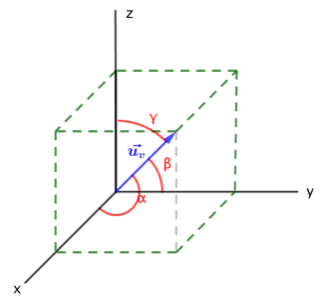
\includegraphics[width=.45\textwidth]{imagenes/imagenes09/T09IM18.png}
\end{figure}
\end{multicols}

\subsection{Distancia entre dos puntos}

\begin{defi}
Dados $A,B \in E_3$ dos puntos del espacio, se define la distancia entre ellos como: $\quad$ \colorbox{LightYellow}{$\; d(A,B)=|\overrightarrow{AB}|\;$}

\noindent \textit{Propiedades}:
$\quad d(A,B)=d(B,A)\; ;  \qquad  d(A,B)=0 \leftrightarrow A=B$.	
\end{defi}

\begin{ejem}
 
\begin{multicols}{2}

Clasifica el triángulo de vértices:
 
$A(3,4,0);\; B(3,0,1); \; C(0,-5,2)$

\begin{figure}[H]
	\centering
	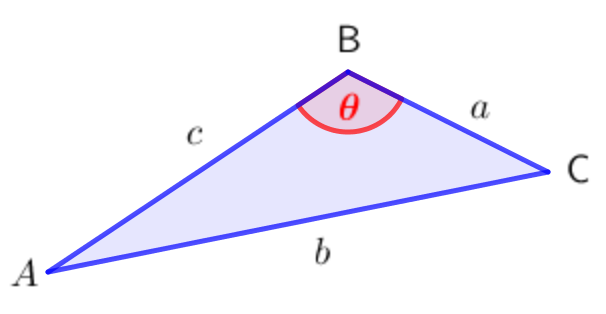
\includegraphics[width=.35\textwidth]{imagenes/imagenes09/T09IM19.png}
\end{figure}
\end{multicols}

$\overrightarrow{AB}=B-A=\;\;(0,-4,1) \to |\overrightarrow{AB}|=\sqrt{0^2+(-4)^2+1^2}=\sqrt{17}\; u=c$

$\overrightarrow{AC}=C-A=(-3,-9,2) \to |\overrightarrow{AB}|=\sqrt{94}\; u=b$

$\overrightarrow{BC}=C-B=(-3,-5,1) \to |\overrightarrow{AB}|=\sqrt{35}\; u=a$

Al ser los tres lados distintos, el triángulo es `escaleno'.

Test de Pitágoras: $\sqrt{94}^2 > \sqrt{35}^2+\sqrt{17}^2 \to$ el triángulo es `obtusángulo' en $B$.

Cálculo del ángulo $B$: $\overrightarrow{BC}=(-3,-5,1)\; \quad \overrightarrow{BA}=-\overrightarrow{AB}=(0,4,-1)$

$\overrightarrow{BC}\cdot \overrightarrow{BA}=(-3,-5,1)\cdot (0,4,-1)=0-20-1=-21$

$|\overrightarrow{BC}|\;|\overrightarrow{BA}|\cos B=\sqrt{35} \sqrt{17} \cos \theta$

Luego, $-21=\sqrt{35} \sqrt{17} \cos \theta \longrightarrow \theta = 149.42^o$. Por lo que el área del triángulo será: $S=\frac 1 2 a c \sin B=\frac 1 2 \sqrt{35} \sqrt{17} \sin 149.42^o= 6.20 u^2$
\end{ejem}

\section{Producto vectorial}

\begin{defi}
El producto vectorial de dos vectores $\vec u$ y $\vec v$ es un nuevo vector $\vec u \times \vec v$	 tal que:

	\begin{multicols}{2}				
	--- su módulo es $|\vec u \times \vec v|=|\vec u||\vec v| \sin \theta $, \small{con $\theta$ el ángulo que forman $\vec u$ y $\vec v$}\normalsize{.}
				
	---  su dirección es perpendicular al plano que forman $\vec u$ y $\vec v$.
				
	---  y su sentido es el de avance del giro de un sacacorchos que intente llevar el vector $\vec u$ hacia el $\vec v$ por el camino más corto.
	
	\begin{figure}[H]
	\centering
	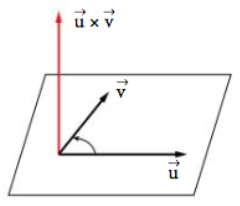
\includegraphics[width=.45\textwidth]{imagenes/imagenes09/T09IM20.png}
	\end{figure}
	\end{multicols}

\end{defi}


\textbf{Propiedades del producto vectorial}

\begin{multicols}{2}


\noindent $\bullet $ El \underline{módulo} del producto vectorial mide el \underline{área del paralelogramo} que forman los vectores $\vec u$ y $\vec v$:

$ |\vec u \times \vec v|=|\vec u||\vec v| \sin \theta$
\begin{figure}[H]
	\centering
	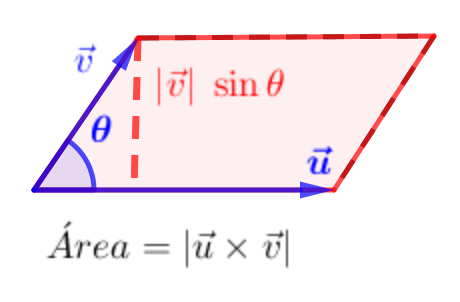
\includegraphics[width=.3\textwidth]{imagenes/imagenes09/T09IM21.png}
	\end{figure}
	\end{multicols}


\begin{itemize}
\item ¡El producto vectorial es \underline{no-conmutativo}!: $\vec u \times \vec v=-\vec v \times \vec u$

		
\vspace{-2mm} \item  $\vec u \times \vec u=\vec 0$
		
\vspace{-2mm} \item  Tomaremos la BON \underline{orientada}, $\vec i \times \vec j = \vec k$; $\vec j \times \vec k = \vec i$ y $\vec k \times \vec i = \vec j$
		
\vspace{-2mm} \item  $(\alpha \vec u)\times \vec v=\alpha (\vec u \times \vec v)= \vec u \times (\alpha \vec v)$
		
\vspace{-2mm} \item  ¡\underline{No} se cumple la \underline{asociativa}!: $\vec u \times (\vec v \times \vec w) \neq (\vec u \times \vec v)\times \vec w$
		
\vspace{-2mm} \item  \underline{Distributivas}: $\vec u \times (\vec v + \vec w)= \vec u \times \vec v + \vec u \times \vec w$; $(\vec u + \vec v)\times \vec w=\vec u \times \vec w + \vec v \times \vec w$
		
\vspace{-2mm} \item  En componentes, el desarrollo del producto vectorial es un determinante:
		
\centerline{\colorbox{LightYellow}{$\; \boldsymbol {\overrightarrow { u } \times \overrightarrow { v } \quad =\quad \left| \begin{matrix} \overrightarrow { i }  & \overrightarrow { j }  & \overrightarrow { k }  \\ u_x & u_y & u_z \\ v_x & v_y & v_z \end{matrix} \right|}\;  $}}

\vspace{-2mm} \item $\vec u \times \vec v$ siempre es un vector perpendicular a $\vec u$ y a $\vec v$ y su módulo representa el área del paralelogramos que definen estos dos vectores.
\end{itemize}
\justify

\begin{figure}[H]
	\centering
	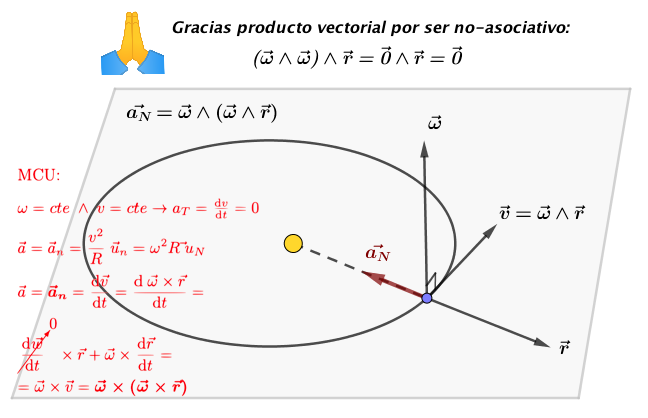
\includegraphics[width=.9\textwidth]{imagenes/imagenes09/T09IM22.png}
	\caption*{Afortunadamente, el producto vectorial no es asociativo.}
	\end{figure}
	
\begin{ejem}
Los tres puntos siguientes forman un triángulo, calcula su área usando el producto vectorial.  $\quad A(3,4,0);\; B(3,0,1); \; C(0,-5,2)$	
\end{ejem}
\begin{multicols}{2}
Consideremos los vectores $\overrightarrow{AB}$ y $\overrightarrow{AC}$, entonces, el módulo del vector producto vectorial de ambos, $|\overrightarrow{AB} \times \overrightarrow{AC}|$, representará el área del paralelogramo y, su mitad, el área del triángulo.

\begin{figure}[H]
	\centering
	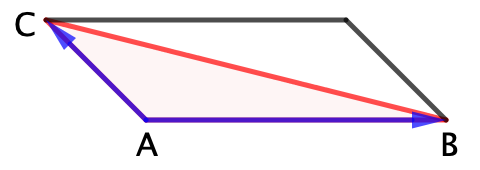
\includegraphics[width=.5\textwidth]{imagenes/imagenes09/T09IM23.png}
	\end{figure}
\end{multicols}

\noindent \textbf{Área del triángulo}  \colorbox{LightYellow}{$\boldsymbol{ABC}$: $\boldsymbol{ A_T=\frac 1 2 |\overrightarrow{AB} \times \overrightarrow{AC}| }$}

\noindent $\overrightarrow{AB}=B-A=(0,-4,1);\qquad \overrightarrow{AC}=C-A=(-3,-9,2)$

\noindent $\overrightarrow{AB} \times \overrightarrow{AC}= \left| \begin{matrix}  \vec i & \vec j & \vec k \\0&-4&1\\-3&-9&2 \end{matrix} \right|= \text{ por adjuntos primera fila (*) }=$

\noindent $=\vec i \; (-1)^{1+1}M_{11}+\vec j \; (-1)^{1+2}M_{12}+\vec k \; (-1)^{1+3}M_{13}=$

\noindent $=\vec i \; \left| \begin{matrix} -4&1\\-9&2 \end{matrix} \right|  +\vec j \; \left| \begin{matrix} 0&1\\-3&2\end{matrix} \right| +\vec k \; \left| \begin{matrix} 0&-4\\-3&-9 \end{matrix} \right|=$

\noindent $=\vec i (-8-(-9)+\vec j (0-(-3))+\vec k (0-12)=\vec i - 3 \vec j - 12 \vec k =(1,-3,-12)$

\noindent $|\overrightarrow{AB} \times \overrightarrow{AC}|=\sqrt{1^2+(-3)^2+(-12)^2}=\sqrt{154}$

\noindent Y el área del triángulo: $A_T=\frac 1 2 \sqrt{154}\simeq 6.20\; u^2$, mismo resultado que el obtenido al final del ejemplo anterior.

\noindent (*) \textcolor{gris}{\small{Es costumbre, en el desarrollo del determinante de un producto vectorial, hacerlo por adjuntos de la primera fila, de este modo, las componentes del vector salen separadas ($\vec i, \vec j, \vec k$), pero también lo hubiésemos podido calcular por Sarrus:}} 

\noindent \textcolor{gris}{\footnotesize{$\overrightarrow{AB} \times \overrightarrow{AC}= \left| \begin{matrix}  \vec i & \vec j & \vec k \\0&-4&1\\-3&-9&2 \end{matrix} \right|= -8 \vec i -3\vec j -(12 \vec k-9 \vec i)=\vec i-3\vec j-12 \vec k=(1,-3,-12) $}\normalsize{.}}

\section{Producto mixto}

\begin{defi}

Dados tres vectores del espacio, $\vec u, \vec v, \vec w \in V_3$, se define el producto mixto de ellos como el producto escalar del primero por el vector que se obtiene como producto vectorial del segundo por el tercero, se representa por $[\vec u, \vec v, \vec w]$.

\vspace{2mm} \centerline{\colorbox{LightYellow}{$\; \boxed{\;[\vec u, \vec v, \vec w]=\vec u \cdot (\vec v \times \vec w)=|\vec u|\cdot|(\vec v \times \vec w)|\cdot \cos \theta\; }\;$}}

\end{defi}
\justify

En componentes, el producto mixto se calcula como un determinante:

\vspace{2mm}\centerline{\colorbox{LightYellow}{$\; [\overrightarrow { u } ,\overrightarrow { v }, \overrightarrow { w }]  \; =\; \left| \begin{matrix} u_{ 1 } & u_{ 2 } & u_{ 3 } \\ v_{ 1 } & v_{ 2 } & v_{ 3 } \\ w_{ 1 } & w_{ 2 } & w_{ 3 } \end{matrix} \right|\; $}}

\vspace{2mm}El producto mixto $[\vec u, \vec v, \vec w]$ mide, en valor absoluto, el volumen del paralelepípedo formado por los tres vectores.

Por propiedades de los determinantes y del valor absoluto podemos afirmar que para el cálculo del volumen de un paralelepípedo formado por tres vectores no importa el orden en que los cojamos para calcular el producto mixto.

\textit{El volumen del prisma es $\boldsymbol{ \frac 1 2 }$ del del paralelepípedo y el de la pirámide $\boldsymbol{ \frac 1 3 }$ del del prisma o $\boldsymbol{ \frac 1 6 }$ del del paralelepípedo.} 


	\begin{figure}[H]
	\centering
	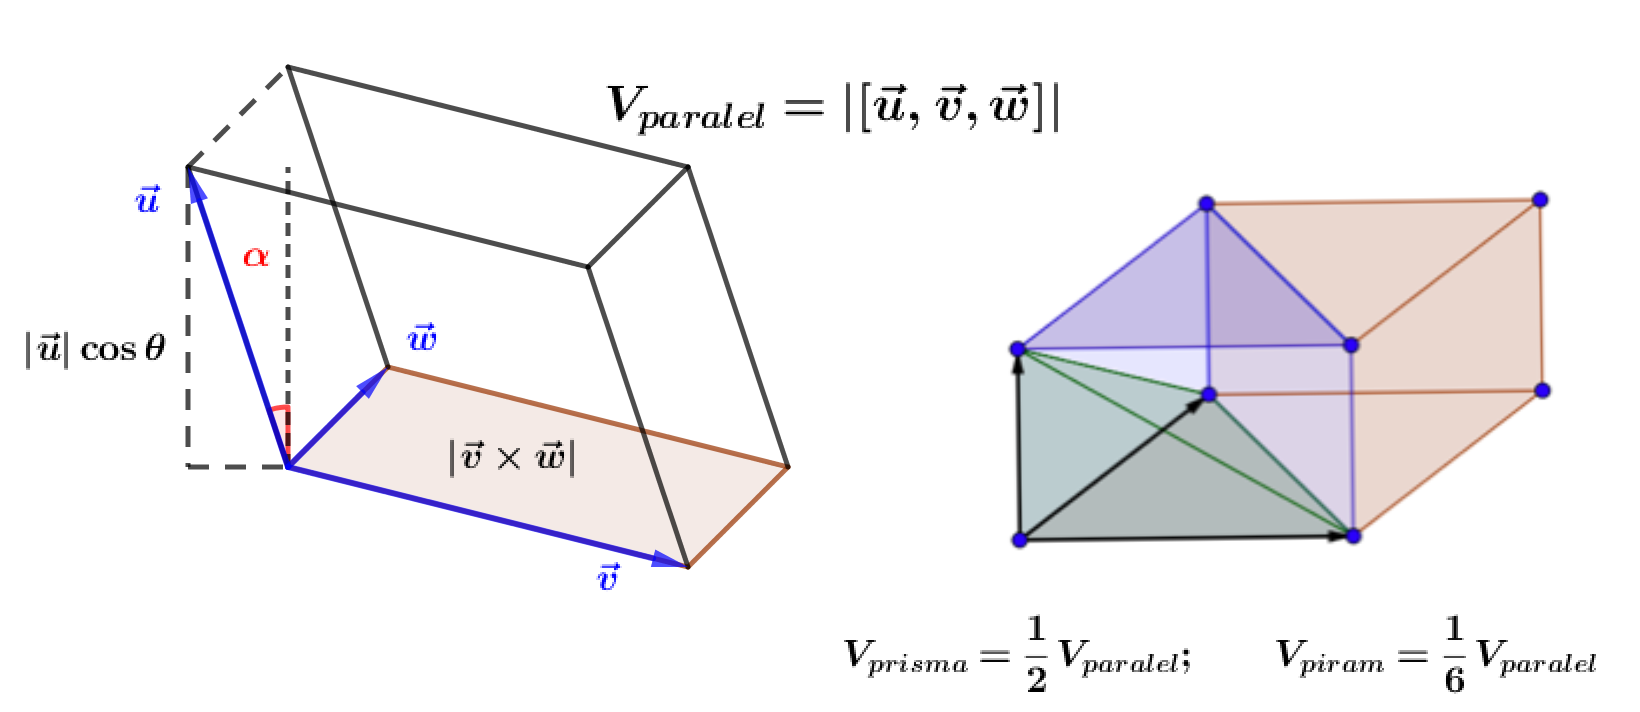
\includegraphics[width=1\textwidth]{imagenes/imagenes09/T09IM24.png}
	\end{figure}
\justify	
\begin{ejem}
Calcula el volumen de la pirámide de vértices: $A(1,2,3),$ $B(0,2,5),$  $C(1,1,-2)$ y $D(2,4,3)$	
\end{ejem}

\noindent Dados los vértices de la pirámide, calculamos los vectores $\overrightarrow{AB}, \overrightarrow{AC}, \overrightarrow{AD}$

\noindent $\overrightarrow{AB}=B-A=(-1,0,-2); \; \overrightarrow{AC}=C-A=(0,1,-5); \; \overrightarrow{AD}=D-A=(1,2,0)$

\noindent $[\overrightarrow{AB}, \overrightarrow{AC}, \overrightarrow{AD}]= \left| \begin{matrix} -1&0&2\\0&1&-5\\1&2&0 \end{matrix} \right|=-12 \to |\; [\overrightarrow{AB}, \overrightarrow{AC}, \overrightarrow{AD}]\;|=|-12|=12$

\noindent El volumen de la pirámide es: $V=\frac 1 6 \; |\; [\overrightarrow{AB}, \overrightarrow{AC}, \overrightarrow{AD}]\;| = \frac 1 6 \; 12=2\; u^3$
	

\section {Ejercicios}

\subsection {Ejercicios resueltos}

\begin{ejre}
	Considera el vector $\vec u=(6,-7,6)$. Encuentra los ángulos que forma este vector con los ejes coordenados y da un vector paralelo a él de módulo $55$
\end{ejre}

\begin{proofw}\renewcommand{\qedsymbol}{$\diamond$}
	Calculemos un vector unitario $\hat u$ en la dirección de $\vec u$:
	
\noindent $|\vec u|=\sqrt{6^2+(-7)^2+6^2}=11 \to \hat u = \frac 1 {|\vec u|}\; \vec u= \frac 1 {11}\; (6,-7,6)=$ 

\noindent $=(6/11,-7/11,6/11)=(\cos \alpha, \cos \beta, \cos \gamma)$ (cosenos directores), siendo $\alpha, \beta, \gamma$ los ángulos que forman tanto $\vec u$ como $\hat u$ (son paralelos) con los ejes coordenados $X,Y,Z$ respectivamente.

\noindent $\alpha=\gamma= arc cos (6/11)=56.94^o; \quad \beta= arc cos (-7/11)=129.52^o$. Luego, $\vec u$ forma un ángulo de $56.94^o$ con el eje $X$, de $129.52^o$ con el eje $Y$ y de $56.94^o$ con el eje $Z$.

\noindent Por otra parte, un vector paralelo a $\vec u$ (también paralelo a $\hat u$) de módulo $55$ será $55\hat u=55 \; \frac 1 {11}\; (6,-7,6)=(30,-35,30)$, si lo queremos del mismo sentido o $(-30,35,-30)$ si lo queremos de sentido contrario. 
\end{proofw}
	
\begin{proofw}\renewcommand{\qedsymbol}{$\diamond$}
	
\end{proofw}

\begin{ejre}
	Sean $\vec a=(4,0,-5); \; \vec b=(-4,3,0);\; \vec c=(-2,-3,5)$, encuentra:
	
	a). La proyección de $\vec a$ sobre $\vec b$.
	
	b). El área del paralelogramos formados por $\vec a$ y $\vec b$.
	
	c). El volumen del paralelepípedo formado por los vectores  $\vec a$ $\vec b$ y $\vec c$.		
	
\end{ejre}

\begin{proofw}\renewcommand{\qedsymbol}{$\diamond$}
a) $Proy_{\;\vec b} \; \vec a= \dfrac {\vec a \cdot \vec b}{|\vec b|}= \dfrac {(4,0,-5)\cdot (-4,3,0)}{|(-4,3,0)|}=\dfrac {-16+0+0}{\sqrt{(-4)^2+3^2+0^2}}=\dfrac {-16}{5}$

\noindent b) $\vec a \times \vec b= \left| \begin{matrix} \vec i & \vec j & \vec k \\4&0&-5\\-4&3&0 \end{matrix} \right|= 15\vec i + 20 \vec j + 12 \vec k =(15,20,12) \to A=|\vec a \times \vec b|=|\;(15,20,12)\;|=\sqrt{15^2+20^2+12^2} =\sqrt{769}\simeq 27.73\; u^2$

\noindent c) $V=abs \left(\;
\left| \begin{matrix} 4&0&-5\\-4&3&0 \\ 2&3&-5 \end{matrix} \right|
\; \right)
=|-30|=30\; u^3$
\end{proofw}

\begin{ejre} Obtén $5$ vectores perpendiculares a $\vec u=(2,-1,7)$, no proporcionales entre sí.
\end{ejre}

\begin{proofw}\renewcommand{\qedsymbol}{$\diamond$}
	Cualquier vector de la forma $\vec v=(\alpha, \beta, \gamma)$ es perpendicular a $\vec u$ si y solo si $\vec u \cdot \vec v=0$.
	
	Tomado $\vec v_1=(0, 7, 1)$, es evidente que  $\vec u \cdot \vec v=(2,-1,7)\cdot (0,7,-1)=0-7+7=0$, por lo que $\vec v_1 \bot \vec u$.
	
	Si hacemos ahora  $\vec v_2=(-7,0,2)$, también es sencillo comprobar que $\vec u \cdot \vec v=0$ y lo mismo ocurre para $\vec v_3=(1,2,0)$. \textcolor{gris}{Para esto, hemos tomado una componente nula en $\vec v_i$ y hemos intercambiado de posición las otras dos de $\vec u$ cambiando el signo a una de ellas.}
	
	Comprobemos que cualquier combinación lineal de éstos, p.e. $\vec v_4=\vec v_1+\vec v_2=(-7,7,3)$ y $\vec v_5=\vec v_1+\vec v_2+\vec v_3=(-6,9,3)$ también son perpendiculares al vector $\vec u$. P.e., $\vec v_5 \cdot \vec u=(-6,9,3)\cdot (2,-1,7)=-12-9+21=0 \to \vec v_5 \bot \vec u$. Dejamos que el/la lector/a compruebe que también $\vec v_4$ es perpendicular a $\vec u$.
	
	\textcolor{gris}{Para encontrar la forma de todos los vectores $\vec v$ perpendiculares a $\vec u$, haríamos que $\vec v \cdot \vec u=(\alpha, \beta, \gamma)\cdot (2,-1,7)=2\alpha-\beta+7\gamma=0 \to$, despejando $\gamma: \quad  \vec v=(\alpha, 2\alpha+7\gamma, \beta),\; \forall \alpha, \gamma \in \mathbb R$}
\end{proofw}


\begin{ejre}
	Dados $\vec u=(1,0,-1); \; \vec v=(2,3,1)$, calcular $\vec u \cdot \vec v$, $|\vec u|$, $|\vec v|$ y él ángulo que forman $\theta =  \widehat{\vec u, \vec v}= \measuredangle \{\vec u, \vec v\} $
\end{ejre}

\begin{proofw}\renewcommand{\qedsymbol}{$\diamond$}
	$\vec u \cdot \vec v=(1,0,-1) \cdot (2,3,1)=1\cdot 2+0\cdot 3+(-1)\cdot 1=2+0-1=1$
	
	\noindent $|\vec u|=\sqrt{1^2+0^2+(.1)^2}=\sqrt{2}; \quad |\vec v|=\sqrt{2^2+3^2+1^2}=\sqrt{14}$
	
	\noindent $\vec u \cdot \vec v = |\vec u|\; |\vec v|\cos \theta \to \cos \theta = \dfrac {\vec u \cdot \vec v}{|\vec u|\; |\vec v|}=\dfrac {1}{\sqrt{2}\; \sqrt{14}} \to $
	
	\noindent $\theta = \text{arc cos} =\dfrac {1}{\sqrt{2}\; \sqrt{14}}= 79.11^o  \;\;\; \textcolor{gris}{\cancel{(280.89^o)}} $
\end{proofw}


\begin{ejre}
	Obtén un vector perpendicular a $\vec u=(3,-1,2)$ y a $\vec v=(1,0,-3)$
\end{ejre}

\begin{proofw}\renewcommand{\qedsymbol}{$\diamond$}
	Dos vectores de distinta dirección (no proporcionales), como $\vec u$ y $\vec v$, forman un `plano vectorial', solo queda una dirección perpendicular posible.
	
\noindent Sea $\vec w=(\alpha, \beta, \gamma)$ el vector buscado:

\noindent Por ser $\vec w$ perpendicular a $\vec u$, ha de ocurrir que 

$\vec u \cdot \vec w=\boldsymbol{ 0}=(3,-1,2)\; ((\alpha, \beta, \gamma)=\boldsymbol{ 3\alpha-\beta+2\gamma}\quad (1*)$ 

\noindent Por ser $\vec w$ perpendicular a $\vec v$, ha de ocurrir que 

$\vec v \cdot \vec w=\boldsymbol{ 0}=(1,0,-3)\; ((\alpha, \beta, \gamma)=\boldsymbol{ \alpha-3\gamma}\quad (1*)$ 

\noindent Con $(1*)$ y $(2*)$, tenemos un SEL homogéneo sencillísimo de resolver: $(2*)\to \alpha=3\gamma \to (1*)\to \beta=11\gamma$. Con lo que los vectores $\vec w$ han de ser de la forma: $\vec w=(3\gamma, 11\gamma, \gamma)\; \; \forall \gamma \in \mathbb R$. Algunos posibles vectores $\vec w$ podrían ser $(3,11,1); \; (-3,-11,-1); \; (33,121,11); \; $ etc.

Otra forma de enfocar el problema es a través del `producto vectorial' ya que $\vec u \times \vec v \; \bot \; \vec u$ y también $\vec u \times \vec v \; \bot \; \vec v$, basta pues con definir $\vec w=\vec u \times \vec v$:

\noindent $\vec w =\vec u \times \vec v=\left| \begin{matrix} \vec i & \vec j & \vec k \\ 3&-1&2 \\ 1&0&-3 \end{matrix} \right|=  \vec i \; \left| \begin{matrix}  -1&2 \\ 0&-3 \end{matrix} \right| \; - 
\vec j \; \left| \begin{matrix}  3&2 \\ 1&-3 \end{matrix} \right| \; +
\vec k \; \left| \begin{matrix}  3&-1 \\ 1&0 \end{matrix} \right| =3\vec i +11\vec j + \vec k=(3,11,1)$ 

\end{proofw}


\begin{ejre}
	Calcula el área de los siguientes triángulos:
	
\noindent \small{$a)\; A(2,3,7); \; B(1,-5,4); C(7,0,11)\quad b)\; P(3,-7,4);\; Q(-1,2,5);\; R(-5,11,6)$}
\end{ejre}

\begin{proofw}\renewcommand{\qedsymbol}{$\diamond$}

Para ambos apartados, formamos los vectores: $\overrightarrow{AB}=B-A=(-1,-8,-3)$;  $\overrightarrow{AC}=(5,-3,4)$;  $\overrightarrow{PQ}=Q-P=(-4, 9, 1)$; $\overrightarrow{PR}=(-8,18,2)$

	\normalsize{--- a)} $A_T=\frac 1 2 |\overrightarrow{AB} \times \overrightarrow{AC} |= \frac 1 2 \; \left|\begin{matrix} \vec i &\vec j & \vec k \\ -1&-8&-3\\5&-3&4\end{matrix} \right|=\frac 1 2 |(-41,-11,43)|=\frac 1 2 \sqrt{3651}\simeq 30.21\; u^2$ 
	
	\noindent \normalsize{--- b)} $A_T=\frac 1 2 |\overrightarrow{PQ} \times \overrightarrow{PR} |= \frac 1 2 \; \left|\begin{matrix} \vec i &\vec j & \vec k \\ -4&9&1\\-8&18&2\end{matrix} \right|=\text{ dos filas proporcionales }=\frac 1 2 \cdot 0=0$ 
	
	\small{\textcolor{gris}{¿Cómo puede ser un triángulo de área cero?. Basta con que los tres puntos estén alineados. En efecto, $P,Q$ y $Q$ están alineados pues los vectores  $\overrightarrow{PQ}$ y  $\overrightarrow{PR}$ tiene las componentes proporcionales $(\; (-8)/(-4)=1/9/=2/1\; )$}}\normalsize{.}
\end{proofw}


\begin{ejre}
	Calcula el volumen de los siguientes tetraedros:
	
	$a)\quad A(-7,-2,5); \; B(0,2,0); \; C(-9,3,8); \; D(-7,5,9)$
	
	$b)\quad A(-7,-2,5); \; B(0,2,0); \; C(-9,3,8); \; D(1,21,4)$
\end{ejre}

\begin{proofw}\renewcommand{\qedsymbol}{$\diamond$}
	Usaremos el producto mixto: $V_T=\frac 1 6\;  |\; [\overrightarrow{AB},\overrightarrow{AC},\overrightarrow{AD}] \;|$, donde $V_T$ será el volumen del tetraedro de vértices $A,B,C \text{ y } D$.
	
\noindent	--- $a)\quad \overrightarrow{AB}=(7,4,-5);\; \overrightarrow{AC}=(-2,5,3); \; \overrightarrow{AD}=(0,7,4)$

\noindent $V=\frac 1 6 \; abs \left( {\left| \begin{matrix} 7&4&-5\\-2&5&3\\0&7&4 \end{matrix} \right|} \right) = \frac 1 6 \;|95|= \frac {95}{6} \; u^3$

\noindent	--- $b)\quad \overrightarrow{AB}=(7,4,-5);\; \overrightarrow{AC}=(-2,5,3); \; \overrightarrow{AD}=(8,23,-1)$

\noindent $V=\frac 1 6 \; abs \left( {\left| \begin{matrix} 7&4&-5\\-2&5&3\\8&23&-1 \end{matrix} \right|} \right) = \frac 1 6 \;|0|= 0 \; u^3$

\textcolor{gris}{¿Cómo puede ser un tetraedro de volumen cero?. Porque no tiene altura (V=1/3 área base * altura), ergo los tres vectores son coplanarios, están en el mismo plano. De otro modo, los 4 puntos son coplanarios y no hay tetraedro.} \textit{El cálculo del volumen del tetraedro formado por cuatro puntos (el producto mixto, un determinante), nos permite decidir si los \colorbox{LightYellow}{cuatro puntos dados son coplanarios $\leftrightarrow$ el volumen del tetraedro es cero}.}
	
\end{proofw}


\begin{ejre}
	Calcula el área total y el volumen del tretraedro de vértices $A(2,3,1)$; $B(4,1,-2)$; $C(6,3,7)$; $D(-5,-4,8)$.

\end{ejre}

\begin{proofw}\renewcommand{\qedsymbol}{$\diamond$}
	$V_{T_{ABCD}}=\frac 1 6\;  |\; [\overrightarrow{AB},\overrightarrow{AC},\overrightarrow{AD}] \;| = \frac 1 6 \; abs \left( { \left| \begin{matrix} 2&-2&-3\\4&0&6\\-7&-7&7  \end{matrix}  \right|  } \right) = \frac {308}{6}=\frac {154}{3}\; u^3$
	
	\begin{multicols}{2}
	\begin{figure}[H]
	\centering
	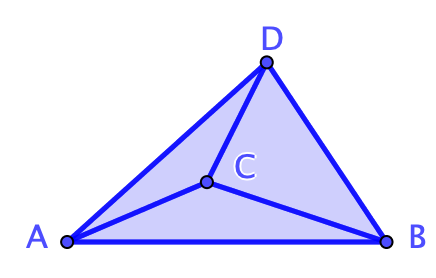
\includegraphics[width=0.5\textwidth]{imagenes/imagenes09/T09IM25.png}
	\end{figure}
	
	En un tetraedros $ABCD$ observamos $4$ triángulos: $ABC$, $ACD$, $BCD$, $ABD$; la suma de sus áreas nos dará el área total. Recordemos que el área de un triángulo es la mitad que la del paralelogramo, p.e., $A_{ABC}=\frac 1 2 \,| \overrightarrow{AB} \times \overrightarrow{AC}|$
	\end{multicols}

\noindent 	$A_{ABC}=\frac 1 2 \,| \overrightarrow{AB} \times \overrightarrow{AC}| = \frac 1 2 \; abs \left( \left| \begin{matrix}  \vec i & \vec j & \vec k \\2&-2&-3\\4&0&6   \end{matrix} \right|  \right)=\frac 1 2 |\;-12 \vec i -24 \vec j + 8 \vec k \; |=\frac 1 2 |(-24,-12,8)|=\frac 1 2 \sqrt{784}=28/2=14 \; u^2$

\noindent 	$A_{ACD}=\frac 1 2 \,| \overrightarrow{AC} \times \overrightarrow{AD}| = \frac 1 2 \; abs \left( \left| \begin{matrix}  \vec i & \vec j & \vec k \\4&0&6\\-7&-7&7   \end{matrix} \right|  \right)=\frac 1 2 |\; 42 \vec i - 70 \vec j - 28 \vec k \; |=\frac 1 2 |(42,-70,-28)|=\frac 1 2 \sqrt{7448}=\sqrt{1862} \; u^2 \simeq 43.15\; u^2$


Compruébese que $A_{BCD}=60.19\; u^2$ y que $A_{ABD}=22.68\; u^2$, por lo que el área total del tetraedro será: $A_{ABCD}=14+43.15+60.19+22.68=140.02\; u^2$

\end{proofw}

	\begin{multicols}{2}
\begin{ejre}.
	
	Calcula la distancia entre los puntos $P$ y $Q$ que aparecen en el siguiente cubo.
	
	\begin{figure}[H]
	\centering
	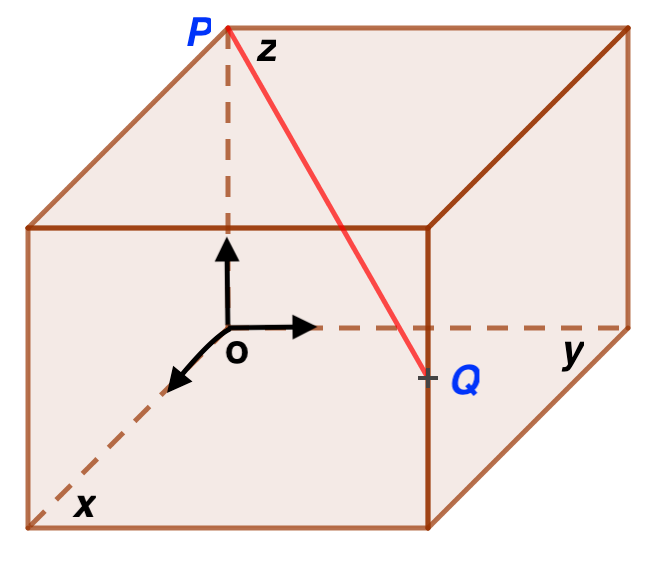
\includegraphics[width=0.3\textwidth]{imagenes/imagenes09/T09IM26.png}
	\end{figure}
	
\end{ejre}
	\end{multicols}
	
\begin{proofw}\renewcommand{\qedsymbol}{$\diamond$}
	Poniendo el origen y con la elección de ejes que aparece en la figura, las coordenadas de los extremos del segmento cuya longitud pretendemos medir (y asumiendo que $Q$ está en el punto medio de una arista), llamando $l$ a la longitud del cubo, son: $P(0,0,l),\; Q(l,l,l/2)$
	
\noindent $\overrightarrow{PQ}=Q-P=(l,l,l/2)-(0,0,l)=(l,l,-l/2)$

\noindent $long(\overline{PQ} )=d(P,Q)=|\overrightarrow{PQ}|=|\; (l,l,-l/2) \;|=\sqrt{l^2+l^2+(-l/2)^2}=\sqrt{9/4 \; l^2}=3/2 \; l\; (u)$.
\end{proofw}

\begin{ejre}
	Los puntos $A(1,2,3)$; $B(-2,2,7)$ y $C(4,6,3)$ definen un triángulo en el espacio. Clasifíquese y calcúlese su área.
	
	El vector $\vec u=(2,-1,5)$ traslada los vértices del triángulo a los puntos $A'$, $B'$ y $C'$ y así se consigue un prisma. Calcúlense las coordenadas de los vértices trasladados y el volumen del prisma.
\end{ejre}

\begin{proofw}\renewcommand{\qedsymbol}{$\diamond$}
	$\overrightarrow {AB}=B-A=(-3,0,4) \to c=|\overrightarrow {AB}|=\sqrt{(-3)^2+0^2+4^2}=5\; u$
	
\noindent $\overrightarrow {AC}=C-A=(3,4,0) \to b=|\overrightarrow {AC}|=\sqrt{3^2+4^2+0^2}=5\; u$

\noindent $\overrightarrow {BC}=C-B=(6,4,-4) \to a=|\overrightarrow {BC}|=\sqrt{6^2+4^4+(-4)^2}\simeq 8.25\; u$

Según los lados, el triángulo es `isósceles'.

\noindent $\overrightarrow {AB} \cdot \overrightarrow {AC}=(-3,0,4) \cdot  (3,4,0)= -9=|\overrightarrow {AB}|\;|\overrightarrow {AC}|\; \cos A=25\cos A \to A=arc cos \frac {-9}{25} \Rightarrow A=110.10^o$

El ángulo que forman los lados iguales del triángulo es de $110,10^o$, por lo que el triángulo es `obtusángulo'. Como los otros dos lados son iguales (isósceles), la amplitud de los mismos será de $\frac 1 2 (180^o -110.10^o) \to B=C=34.95^o$

El área del triangulo $ABC$ la obtenemos a través del producto vectorial como:

\noindent $\overrightarrow {AB}\times \overrightarrow {AC}= 
\left| \begin{matrix} \vec i&\vec j&\vec k \\-3&0&4\\3&4&0\end{matrix} \right|=-16\vec i+12 \vec j- 12 \vec k=(-16,12,-12)$

\noindent $|\; \overrightarrow {AB}\times \overrightarrow {AC}\; |=|\; (-16,12,-12)\;| = \sqrt{(-16)^2+12^2+(-12)^2}\simeq 23.32$

\noindent $A_{ABC}=\frac 1 2 \; |\; \overrightarrow {AB}\times \overrightarrow {AC}\; |=\frac 1 2 \; 23.32=11.66 \; u^2$

\begin{multicols}{2}
\begin{figure}[H]
	\centering
	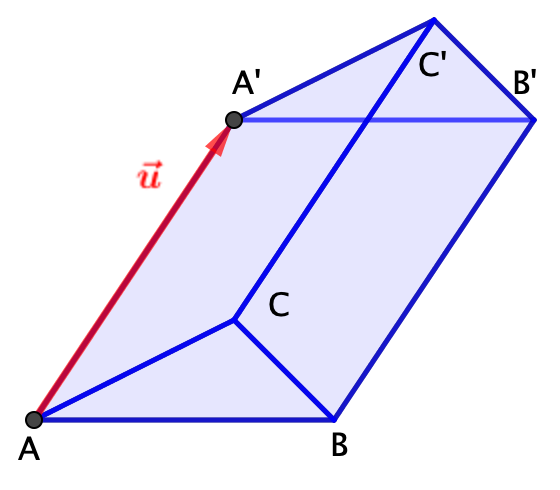
\includegraphics[width=0.4\textwidth]{imagenes/imagenes09/T09IM28.png}
	\end{figure}

Los vectores trasladan puntos:

$A'=A+\vec u =(1,2,3)+(2,-1,5)=(3, 1, 8)$; 

$B'=B+\vec u=(-2,2,7)+(2,-1,5)=(0,1,12)$ y 

$C'=C+\vec u=(4,6,3)+(2,-1,5)=(6,5,8)$
\end{multicols}
Podemos considerar el prisma como el formado por los vectores  $\overrightarrow {AB}$, $\; \overrightarrow {AC}$ y $\overrightarrow {AA'}$, siendo $\overrightarrow {AB'}=A'-A=(2,-1,5) \textcolor{gris}{(=\vec u \text{ evidentemente.)}}$. Su volumen (medio paralelepípedo) lo dará el producto mixto.

\noindent $V_P=$\small{$\frac 1 2\;|\;[\overrightarrow {AB}, \overrightarrow {AC},\overrightarrow {AA'}]\;|=\frac 1 2 \; abs \left(\; \left| \begin{matrix} -3&0&4\\3&4&0\\2&-1&5 \end{matrix} \right| \;\right)$}\normalsize{$=$}$\frac 1 2 \; |-104|=52 \; u^3$
\end{proofw}

\begin{ejre}
	\underline{Aplicación física}: El trabajo $W(J)$ que ejerce una fuerza  constante $\vec F(N)$ sobre un cuerpo para desplazarlo desde una posición inicial $\vec x_0$ a una final $\vec x$ se define como el producto escalar de la fuerza aplicada al cuerpo por el desplazamiento producido,  $W=\vec F \cdot \overrightarrow {\Delta x}$, siendo $\overrightarrow{\Delta x} \; (m)$ el vector desplazamiento, que se calcula como  $\overrightarrow{\Delta x}=\vec x - \vec x_0$.
	
	Calcula el trabajo que ejerce una fuerza constante $F=(\; 3\vec i - 2 \vec j + 4 \vec k \;) \; (N)$cuando desplaza a un cuerpo desde la posición inicial $\vec x_0=(1,1,1) $ a la posición $\vec x=(1,-1,3)$.
\end{ejre}

\begin{proofw}\renewcommand{\qedsymbol}{$\diamond$}
	 $\overrightarrow{\Delta x}=\vec x-\vec x_0=(1,-1,3)-(1,1,1)=(0,-2,2) \; (m) \to W=\vec F \cdot \overrightarrow {\Delta x}=(3,-2,4)\cdot (0,-2,2)=0+4+8=12\; J$
\end{proofw}

\begin{ejre}
	\underline{Aplicación física}: Cuando una carga $q$ entra en un campo magnético $\vec B$ con una velocidad $\vec v$ se ve sometida a la `fuerza de Lorentz' $F=q\, \vec v \times \vec B$.  
	
	Encuentra la fuerza de Lorentz que el campo magnético $\vec B=(1,2,3)\; (T)$ ejerce sobre un electrón ($q=1.6 \times 10^{-19} \; (C)$) cuando accede con una velocidad $\vec v=(1,-1,1)\; (m\cdot s^{-1})$.
\end{ejre}

\begin{proofw}\renewcommand{\qedsymbol}{$\diamond$}
	$F=q\, \vec v \times \vec B=1.6 \times 10^{-19}\; \left| \begin{matrix} \vec i & \vec j & \vec k \\ 1&2&3 \\ 1&-1&1 \end{matrix} \right|= 1.6 \times 10^{-19} (\;5  \vec i + 2 \vec j - 3 \vec k \; )\; (N)$
	
\noindent $|\vec F|= 1.6 \times 10^{-19} \; \sqrt{5^2+2^2+(-3)^2}=6.08 \times 10^{-18}\; N$
\end{proofw}





\subsection{Ejercicios propuestos}

\begin{enumerate}

\item Sean $A(1,2,3); B(5,1,-1); C(-7,\lambda,11)$. Calcula: $\; d(A,B)$; $\lambda$ para que $A$, $B$ y $C$ estén alineados, el punto medio de $\overline{AB}$; $B'$, el simétrico de $B$ respecto de $A$. ¿Cuál debería ser el punto $D$ para que $G=0,-1,2)$ fuese el baricentro del triángulo $ABD$?

\vspace{2mm}
\rightline{\textcolor{gris}{\footnotesize{Solución: $3;\; \lambda=4; \; M_{AB}(3,3/2,1);\; B'(7,5,5); \; D(-6,-6,4)$ }\normalsize{.}}}

\item ¿Cuál de los siguientes vectores tienen la misma dirección? $\vec x=(1,-3,2)$; $\vec y=(2,0,1)$; $\vec z=(-2,6,-4)$; $\vec u=(5,-15,10)$; $\vec v=(10,-30,5)$

\vspace{2mm}
\rightline{\textcolor{gris}{\footnotesize{Solución: $\vec x, \vec z, \vec u$ tienen la misma dirección (paralelos)}\normalsize{.}}}

\item Sean $\vec u=-2\vec i+3\vec j+\vec k$; $\vec v=4\vec i-3\vec j+3\vec k$; $\vec w=-\vec j+4\vec k$. Calcula:
\begin{multicols}{2}
\begin{enumerate}[a) ]
\item $|\;\vec u - \vec v\;|$
\item $\vec u - 3\vec v+2\vec w$
\item $(\vec u -2\vec v)\cdot 3\vec w$
\item $-(4\vec v-3\vec w)\times 2\vec v$
\item Ángulo de $\vec u$ con los ejes coordenados.
\item Ángulo entre $3\vec v$ y $-2\vec w$
\item Volumen de la pirámide que forman los tres vectores.
\end{enumerate}
\end{multicols}
\vspace{2mm}
\rightline{\textcolor{gris}{\tiny{Solución: $a)\; 8.7;\;\; b)\; (-14,10,0);\;\; c) -87;\;\; (54,96,24);\;\; e)\; 122^o_x; \; 36^o_y;\; 74^o_z;\;\; 128.6^o;\; \; 34\; u^3 $}\normalsize{.}}}

\item Considera los vectores $\vec u=(1,-5,2)$; $\vec v=(3,4,-1)$; $\vec w=(5,-2,1)$ y $\vec t=(24,-26,-6)$. Determina $\alpha$, $\beta$ y $\gamma$ para que se cumpla:  
$  \vec t = \alpha \vec u + \beta \vec v + \gamma \vec w$.

\vspace{2mm}
\rightline{\textcolor{gris}{\footnotesize{Solución: $\alpha=6; \; \beta = -2; \; \gamma =4$}\normalsize{.}}}

\item Dados los vectores $\;\vec u=(5,-1,2)\;$ y $\;\vec v=(-1,2,-2)\;$, calcula: $\; \vec u \cdot \vec v;\; |\vec u|;\; |\vec v|;\;$ la proyección de $\vec u$ sobre $\vec v$ y el ángulo que forman $\widehat{\vec u, \vec v }\;$; el valor de $\lambda$ para que el vector $(7,2,\lambda)$ sea perpendicular a $\vec u$. 

\vspace{2mm}
\rightline{\textcolor{gris}{\footnotesize{Solución: $-11; \; 5.48;\; 3; \; -11/3; \; 132^o; \; \lambda=-33/2$}\normalsize{.}}}

\item Dados $\vec u=(3,7,-6)$ y $\vec v =(4,1,-2)$, encuentra un vector perpendicular a $\vec u$ y perpendicular a $\vec v$, cuya primera componente sea $2$.

\vspace{2mm}
\rightline{\textcolor{gris}{\footnotesize{Solución: $[\;\vec w=k\cdot (\vec u \times \vec v)\;] ; \quad (2,9/2,25/4)$ }\normalsize{.}}}

\item Dados $\vec u=(1,-1,0)$ y $\vec v=(2,0,1)$, encuentra un vector $\vec w$ perpendicular a ambos vectores y de módulo $\sqrt{24}$

\vspace{2mm}
\rightline{\textcolor{gris}{\footnotesize{Solución: $\vec w=\pm(-2,-2,4)$ }\normalsize{.}}}

\item $\vec u=(1,2,3); \; \vec v=(-3,0,4)$. Encuentra el vector de proyección de $\vec u$ sobre $\vec v$

\rightline{\textcolor{gris}{\footnotesize{Solución: $[\; \overrightarrow{Proy}_{\;\vec v}\;(\vec u)=\left(Proy_{\;\vec v}\; (\vec u) \right)\; \widehat u=\frac {\vec u \cdot \vec v}{|\vec v|}\; \widehat u= \frac {\vec u \cdot \vec v}{|\vec v|}\; \frac {1}{\vec v} \; \vec v\; ] \;\to \; \frac {9}{25}\; (-3,0,4)$ }\normalsize{.}}}

\item  Para $\vec u=(1,2,2)$ y $\vec v=(-4,5,-3)$, calcula:
\begin{multicols}{2}
\begin{enumerate}[a) ]
\item $\vec u \cdot \vec v$
\item $|\vec u|$ y $|\vec v|$
\item $\widehat{\vec u, \vec v}$
\item $(\vec u + \vec v)\cdot(\vec u-\vec v)$
\item $\vec u \times \vec v$
\item $|\vec u \times \vec v|$
\item Proyección de $\vec u$ sobre $\vec v$
\item El vector de proyección de $\vec v$ sobre $\vec u$
\item $\vec u \times (\vec u \times \vec v)$
\end{enumerate}
\end{multicols}

\rightline{\textcolor{gris}{\tiny{Solución: $a)\; 0;\; \; b)\; 3 y 7.1; \; \; c)\; 90^o; \; \; d)\; -41; \; \; e)\; (-16,-5,-13); \; \; f)\; 15\sqrt{2};\;\;g)\; 0;\;\; h)\; \vec 0\;\;\; i)\; (36,-45,27) $}\normalsize{.}}}


\item Encuentra $t$ para que los vectores $\vec u=(7,4,2)$; $\vec v=(1,14,0)$ y $\vec w=(3,-5,t)$ sean coplanarios \textcolor{gris}{el volumen del paralelepípedo que determinan sea cero}.

\vspace{2mm}
\rightline{\textcolor{gris}{\footnotesize{Solución: $t=1$ }\normalsize{.}}}

\item Sean $\vec u=\vec i+m\vec j+\vec k$ y $\vec v=-2\vec i+4\vec j+m\vec k$. Encuentra el valor de $m$ para que los vectores sean a) paralelos y b) perpendiculares.

\vspace{2mm}
\rightline{\textcolor{gris}{\footnotesize{Solución: $a)\; m=-2; \quad b)\; m=2/5$ }\normalsize{.}}}

\item Los vectores directores de $\vec u$ son $\cos \alpha=0.2$; $\cos. \beta=0.31$ y $\cos \gamma=0.93$, si $|\vec u|=6$, ¿cuáles son sus componentes?

\vspace{2mm}
\rightline{\textcolor{gris}{\footnotesize{Solución: $[\;\vec u=|\vec u|\cdot \widehat u; \;\; \widehat u=(\cos \alpha, \cos \beta, \cos \gamma) \; \to \;]\;\; \vec u=/1.2, 1.86, 5.58)$ }\normalsize{.}}}

\item Dos vectores $\vec u$ y $\vec v$ son tales que $|\vec u|=4$; $|\vec v|=5$ y $|\vec u + \vec v|=7$. ¿Qué ángulo forman?

\vspace{2mm}
\rightline{\textcolor{gris}{\footnotesize{Solución: $78.5^o$}\normalsize{.}}}

\item Los vértices de un triángulo son $A(m,2,-1)$, $B(5,3,-4)$ y $C(7,m,-2)$. Calcula el valor de $m$ para que el triángulo sea rectángulo en $B$ y determina su área.

\vspace{2mm}
\rightline{\textcolor{gris}{\footnotesize{Solución: $\overrightarrow{BA} \bot \overrightarrow{BC} \to m= 1; \; \text{ (área=prod.catetos/2) } \; \sqrt{312}/2\; u^2$ }\normalsize{.}}}

\item Demuestra que $A(t,2,t); B(2,-t,0) \text{ y } C(t,0,t+2)$ son los vértices de un triángulo isósceles. Para $t=2$ calcula su área.

\vspace{2mm}
\rightline{\textcolor{gris}{\footnotesize{Solución: $[\;|\overrightarrow{AB}|; \; |\overrightarrow{AC}|; \; |\overrightarrow{BC}| \;] \; \to$ isósceles en $B; \quad t=2 \to \text{ área }=6\; u^2$}\normalsize{.}}}

\item Dados $P(1,3,-1)$; $Q(a,2,0)$; $R(1,5,4)$ y $S(2,0,2)$, calcula $a$ para que: a) los cuatro puntos sean coplanarios; b) el volumen del tetraedros de vértices $PQRS$ sea $7\;u^3$.

\vspace{2mm}
\rightline{\textcolor{gris}{\footnotesize{Solución: $a)\; a=4/3; \quad b) \; a=10/3 \; \vee \; a=-2/3$}\normalsize{.}}}

\item Dados $P(1,2,1)$; $Q(2,3,1)$; $R(0,5,3)$ y $S(-1,4,3)$, prueba que están en un mismo plano, demuestra que el polígono $PQRS$ es un rectángulo y calcula su área.

\vspace{2mm}
\rightline{\textcolor{gris}{\footnotesize{Solución: $ V_{PQRS}=0\; u^3; \quad \overrightarrow{PQ} \bot \overrightarrow{PS} \text{ y } \overrightarrow{PQ} \bot \overrightarrow{QR}; \quad A_{PQRS}=\sqrt{24} \; u^2$ }\normalsize{.}}}

\item Dados los vectores $\vec u=(-1,2,3)$ y $\vec v=(2,0,-1)$, se pide:

a) Encuentra un vector $\vec w_1$  que sea ortogonal a $\vec u$ y $\vec v$, unitario y cuya tercera componente sea positiva.

b) Encuentra un vector $\vec w_2$ que sea combinación lineal de $\vec u$ y $vec v$ y que sea ortogonal a $\vec v$

\vspace{2mm}
\rightline{\textcolor{gris}{\footnotesize{Solución: $a)\; \vec w_1=\frac {1}{3\sqrt{5}}\; (2,-5,4); \quad b)\; \vec w_2=(t,2t,2t)=(1,2,2) \text{ p.e.}$}\normalsize{.}}}


\item Dados $\vec u=(1,2,3)$ y $\vec v=(1,-1,1)$ encuentra el vector $\vec w$ sabiendo que es ortogonal a $\vec u$ y $\vec v$ y que $[\vec w, \vec u, \vec v]=114$

\vspace{2mm}
\rightline{\textcolor{gris}{\footnotesize{Solución: $\vec w=(15,6,-9)$}\normalsize{.}}}

\item Dados $\vec u=(0,1,2)$ y $\vec v=(1,-1,0)$ y $\vec w=(m+1.2m,2-3m)$, encuentra el valor de $m$ para que
\begin{multicols}{2}
\begin{enumerate}[a) ]
\item $vec u$, $\vec v$ y $\vec w$ sean coplanarios.
\item $\vec w$ sea ortogonal a $\vec u$ y a $\vec v$
\item el volumen de la pirámide formada por los tres vectores sea $3\; u^3$
\end{enumerate}
\end{multicols}

\vspace{2mm}
\rightline{\textcolor{gris}{\footnotesize{Solución: $a)\; m=0; \; \; b)\; m=1; \; \; c)\; m=\pm2$}\normalsize{.}}}

\item Encuentra un vector $\vec u$ que tenga la misma dirección que el vector $\vec v=(1,-2,3)$ y que determine con el vector $\vec w$ un paralelogramo de área $25 \; u^2$

\vspace{2mm}
\rightline{\textcolor{gris}{\footnotesize{Solución: $\vec u=\pm \sqrt{5}\; (1,-2,3)$}\normalsize{.}}}

\item Encuentra un vector $\vec a$ que sea coplanario con $\vec u=(2,-1,1)$ y $\vec v=(1,0,3)$, ortogonal a $\vec w=(2,3,0)$ y cuya primera componente sea $6$ 

\vspace{2mm}
\rightline{\textcolor{gris}{\footnotesize{Solución: $[\;\vec a = k(\vec u \times \vec v)\;; \; \; \vec a\cdot \vec w=0 \;]\; \to\;\vec a=(6,-4,-2))$}\normalsize{.}}}

\item Encuentra un vector $\vec w$ de módulo $10$, perpendicular a $\vec u=(-3,1,0)$ y que forme un ángulo de $60^o$ con $\vec v=(0,10,1)$

\vspace{2mm}
\rightline{\textcolor{gris}{\footnotesize{Solución: $\vec w=(\alpha,\beta,\gamma) \to \vec w_1=\left(\sqrt{\frac {15}{2}}, 3\sqrt{\frac {15}{2}},5 \right); \; \vec w_2=\left(\sqrt{-\frac {15}{2}}, -3\sqrt{\frac {15}{2}},5 \right)$}\normalsize{.}}}

\end{enumerate}

\subsection{Cuestiones}

\begin{enumerate}[Q1. ]

\item Si $\vec u \cdot \vec v=\vec u \cdot \vec w$, ¿se puede asegurar que $\vec v=\vec w$?


\rotatebox{180}{\leftline{\textcolor{gris}{\scriptsize{\hspace{5mm}  Sol: No,  $\vec u=(3,4,0);\; \vec v=(4,0,5); \;  \vec w=(0,3,-1)$ }}}}


\item Demuestra que si $\vec u \;\bot \;\vec v\; $ y $\; \vec u\; \bot \;\vec w \longrightarrow \vec u \; \bot \;(\alpha \vec v + \beta \vec w)$


\rotatebox{180}{\leftline{\textcolor{gris}{\scriptsize{\hspace{5mm}  Sol: Calcula,  $\vec u \cdot (\alpha \vec v + \beta \vec w)$ }}}}


\item Sabiendo que $\;[\vec u, \vec v, \vec w]=0\;$, se puede asegurar con seguridad que:
\begin{multicols}{2}
\begin{enumerate}[a) ]
\item Al menos uno de los tres vectores es el vector $\vec 0$.
\item Los tres vectores son linealmente dependientes, es decir, son coplanarios.
\item El vector $\vec w$ se puede escribir como combinación lineal de los otros dos.
\item Por lo menos, dos de los vectores tienen la misma dirección.
\end{enumerate}
\end{multicols}

\rotatebox{180}{\leftline{\textcolor{gris}{\scriptsize{\hspace{5mm}  Sol: La respuesta correcta es la b). }}}}

\item Sean $\vec u=\left( -\frac 1 {\sqrt{2}},.1,\frac {\sqrt{2}}2\right); \;\; \vec v=\left( -\frac {\sqrt{2}}2, -1,-\frac 1 {\sqrt{2}} \right)$

\begin{multicols}{2}
\begin{enumerate}[a) ]
\item Los vectores tienen el mismo módulo.
\item Son ortogonales.
\item Forman un ángulo de $60^o$.
\item Tienen la misma dirección
\end{enumerate}
\end{multicols}
Elige las respuestas correctas.

\rotatebox{180}{\leftline{\textcolor{gris}{\scriptsize{\hspace{5mm}  Sol: Las respuestas correctas son la a) y la c) }}}}

\item Demuestra que si $\; \vec u \;,\; \vec v\; $ y $\;\vec w\;$ son perpendiculares dos a dos, el producto escalar $\;(\vec u+\vec v)\cdot(\vec w+\vec u)\;$ no puede ser negativo.


\rotatebox{180}{\leftline{\textcolor{gris}{\scriptsize{\hspace{5mm}  Sol: Calcula el producto escalar pedido. }}}}

\item Si $\vec u$ y $\vec v$ son dos vectores que verifican $|\vec u \cdot \vec v|=|\vec u|\;|\vec v|$, ¿qué puedes decir del ángulo que forman?


\rotatebox{180}{\leftline{\textcolor{gris}{\scriptsize{\hspace{5mm}  Sol: $\cos \theta = \pm 1 \to \theta = 0^o \; \vee \theta = 180^o$. }}}}

\item Dados $\vec u$ y $\vec v$ dos vectores no nulos tales que $\vec u \times \vec v=\vec 0$, ¿cómo son los vectores $\vec u$ y $\vec v$?

\rotatebox{180}{\leftline{\textcolor{gris}{\scriptsize{\hspace{5mm}  Sol: $\sin \theta=0 \to  \theta = 0^o \; \vee \theta = 180^o$, vectores paralelos.}}}}

\end{enumerate}

\newpage
\section{Resumen}

\begin{myalertblock}{Resumen de vectores}

\begin{figure}[H]
	\centering
	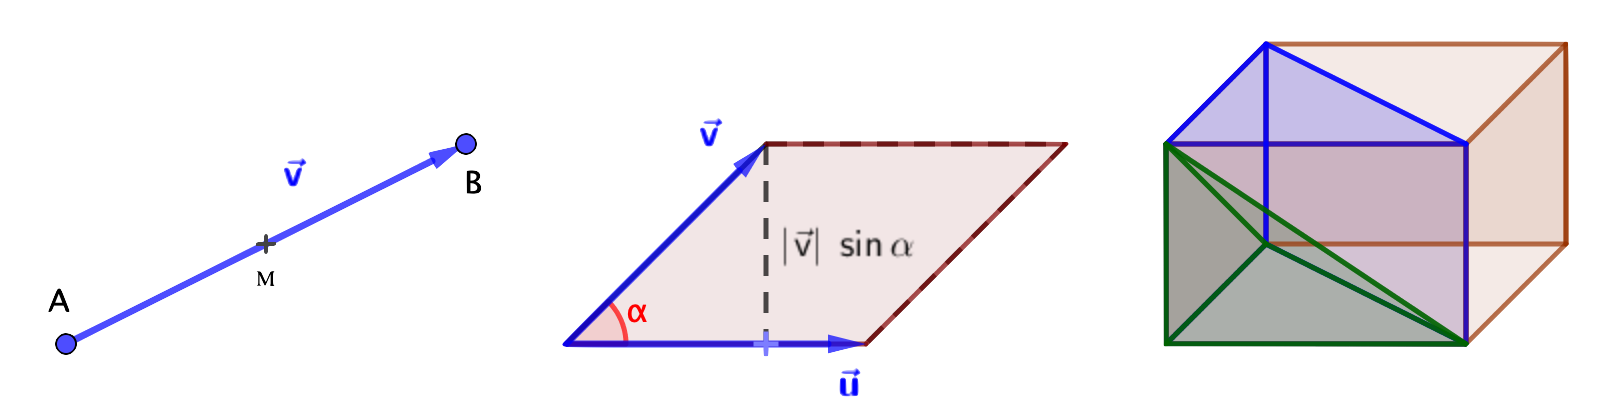
\includegraphics[width=.95\textwidth]{imagenes/imagenes09/T09IM30.png}
\end{figure}

$\vec v=\overrightarrow{AB}=B-A; \quad A+\vec v=B;\quad d(A,B)=|\overrightarrow{AB}|;\quad M=\frac {A+B}{2}$

\vspace{3mm} PRODUCTO ESCALAR: $\quad \boxed{\;\vec u\cdot \vec v= |\vec u|\;|\vec v|\; \cos \theta\;} \quad \in \mathbb R$

\vspace{1mm} \hspace{10mm} $\forall \; \vec u , \vec v \neq \vec 0 \;\longrightarrow \;\; \vec u \;\bot\; \vec v \;\leftrightarrow\; \vec u \cdot \vec v = \vec 0$

\vspace{1mm} \hspace{10mm} --- Módulo de un vectore: $\;|\vec u|\;=\; +\sqrt{\vec u \cdot \vec u}$

\vspace{1mm} \hspace{10mm} --- Ángulo entre dos vectores: $\; \cos \theta=\dfrac{\vec u \cdot \vec v}{|\vec u|\;|\vec v|}$

\vspace{1mm}  \footnotesize{PE en una BON:  $\; \vec u \cdot \vec v=(u_x,u_y.u_z) \cdot (v_x,v_y,v_z)=u_xv_x+u_yv_y+u_zv_z\ \in \mathbb R$}\normalsize{.}

\vspace{3mm} PRODUCTO VECTORIAL: \tiny{(Anticonmutativo)} \normalsize{$\; \vec u \times \vec v = \left| \begin{matrix} \vec i& \vec j& \vec k\\ u_x&u_y&u_z\\v_x&v_y&v_z\end{matrix} \right|$}

\vspace{1mm} \hspace{10mm} $\vec u \times \vec v \; \bot \; \vec u \quad \wedge \quad  \vec u \times \vec v \; \bot \; \vec v $

\vspace{3mm} PRODUCTO MIXTO: $\; [\vec u, \vec v , \vec w]=\vec u\cdot (\vec v \times \vec w) = |\vec u|\cdot |\vec v \times \vec w|\; \cos \alpha$

\vspace{1mm} \hspace{10mm} $\; [\vec u, \vec v , \vec w]= \left| \begin{matrix}  u_x&u_y&u_z\\v_x&v_y&v_z\\w_x&w_y&w_z\end{matrix} \right|$

\vspace{1mm} \small{En valor absoluto, el producto mixto mide el volumen del paralelepípedo que forman los tres vectores. El prisma tiene la mitad del volumen y la pirámide o tetraedros, la sexta parte}\normalsize{.}
\end{myalertblock}


	
	%\begin{figure}[H]
		%\centering
		%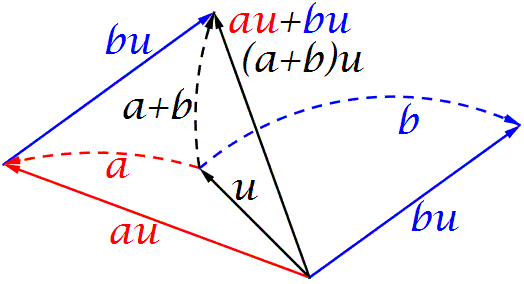
\includegraphics[width=0.5\textwidth]{imagenes/imagenes01/T01IM01.png}
	%\end{figure}
		
%varios párrafos encuadrados - explicaciones ad hoc
%\centering{
%\fbox{
%\parbox{0.95\textwidth}{
%varios
%
%$parrafos
%
%dentro
%}
%}
%}
% \justify


%\rotatebox{180}{\leftline{\textcolor{gris}{tararí}}}.